\documentclass[12pt]{article}
\textwidth=17.5truecm  \voffset=-2truecm
\textheight=23.5truecm \hoffset=-2.5truecm
\setlength{\parindent}{0pt}
\usepackage[bottom]{footmisc}
\usepackage{amssymb}
\usepackage{mathtools}
\usepackage{amsfonts}
\usepackage{graphicx}
\graphicspath{{./figs/}}
\usepackage{color}
\usepackage{float}
\usepackage[hidelinks]{hyperref}
\usepackage{siunitx}
\usepackage[dvipsnames]{xcolor}
\usepackage{caption}
\captionsetup{font=footnotesize}
\usepackage[superscript,biblabel,nomove]{cite}
\usepackage{listings}
\lstset{breaklines=true}
\lstset{basicstyle=\fontsize{8}{10}\ttfamily}
\lstset{framesep=5pt}

\usepackage{mathtools}
\bibliographystyle{unsrt}

%\usepackage{xcolor}
%\pagecolor[rgb]{0,0,0} %black
%\color[rgb]{0.8,0.8,0.8} %grey

\makeatletter
\renewcommand{\@citess}[1]{\textsuperscript{\,[#1]}}
\DeclareRobustCommand{\abs}{\@ifstar\star@abs\normal@abs}
\newcommand{\star@abs}[1]{\left|#1\right|}
\newcommand{\normal@abs}[2][]{\mathopen{#1|}#2\mathclose{#1|}}
\makeatother

%\title{Sequences of real and complex numbers}

\title{%
	Sequences of Real and Complex Numbers \\
	\small Analysis of the Möbius sequence, the logistic map, and sequences of the form $z_{n+1}={z_n}^2+c$}
\author{Dylan Callaghan}
\begin{document}
%\maketitle

	\begin{titlepage}
		\begin{center}
			\vspace*{1cm}
			
			\Huge
			\textbf{Sequences of Real and Complex Numbers}
			
			\vspace{0.5cm}
			\normalsize
			Analysis of the Möbius sequence, the logistic map, and sequences of the form $z_{n+1}={z_n}^2+c$
			
			\vspace{1.5cm}
			
			\textbf{Dylan Callaghan}
			
			\vfill
			
			
			\vspace{0.8cm}
			
			\normalsize
			Nuffield Researchers Project (2020)\\
			dylanrobcallaghan@gmail.com\\
			31\textsuperscript{st} August, 2020
			
		\end{center}
	\end{titlepage}

\newpage
\tableofcontents
\newpage
\section*{Introduction}\label{s_int}
In this report, I will be investigating sequences of both real and complex numbers through topics such as Möbius sequences, period doubling sequences and iterative sequences of complex numbers. Before continuing further, it is important to first understand the definition of a sequence; a sequence is an ordered list of objects in which a value can appear multiple times. There are many types of sequence such as arithmetic and geometric sequences -- these define the rule used to arrive at the next term. In our case, the next term of the sequence is defined by a rule that uses the previous term in the sequence -- this is called a recurrence relation sequence. \\\\
In \S\ref{s_mob}, I will be exploring Möbius sequences - these sequences take the form 
	\[x_{n+1}=\frac{ax_n+b}{cx_n+d}\] 
with a starting $x_0$ value that is then placed back inside the sequence in order to compute the next value. I will explore how the behaviour of this sequence changes based on the parameters $a,\;b,\;c$ and $d$ \\\\
In \S\ref{s_per} I will be exploring the period doubling sequence (the logistic map in this case). This takes the form
	\[x_{n+1} = rx_n(1-x_n)\]
 will be focusing mostly on what values the sequence approaches as the parameter $r$ changes and exploring the connections this has to cycles similar to what we will see in \S\ref{s_mob}.\\\\
Finally in \S\ref{s_zn} I will be looking into the behaviour of the complex sequence $z_{n+1} = {z_n}^2+c$ and linking this to the theory of keep sets and escape sets when choosing both real and complex starting values for $z_0$.\\\\
We will likely find similar behaviours in all 3 topics -- especially when looking at the cyclic behaviour of sequences.
\newpage
\section{Möbius Sequences}\label{s_mob}
I will first begin this section by outlining the Möbius function
\[f(x) = \frac{ax+b}{cx+d}\]
and the Möbius sequence, which is very similar to it but with the recurrence element added, which is as below 
	\[x_{n+1} = \frac{ax_n+b}{cx_n+d}\]
where in both cases $\{a, b, c, d \in \mathbb{R}\}$ The Möbius sequence is always given a starting $x$ value, $x_0$ to calculate the next value of the sequence\footnote{the starting value in this section is always $x_0=1$ unless stated otherwise}. \\
We can see through inspection of the Möbius function that there are horizontal and vertical asymptotes at $y=\frac{a}{c}$ and $x=-\frac{d}{c}$ respectively, with an example on Figure \ref{fig:mobAsymp} showing the function.
	\begin{figure}[H]
		\begin{minipage}{0.725\textwidth}
			\hfill
			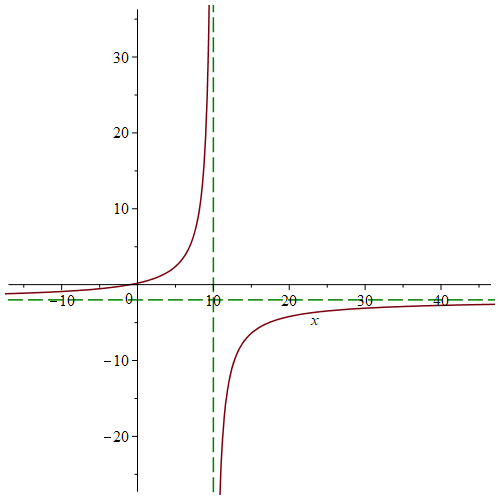
\includegraphics[scale=0.4]{mobAsymp.png}
		\end{minipage}
	\hfill
		\begin{minipage}{0.2\textwidth}
			$a=2,\\b=2,\\ c=-1,\\ d=10\\$
		\end{minipage}
	\caption{Asymptotes of a Möbius function}
	\label{fig:mobAsymp}
	\end{figure}
We can see the function here in red -- with the green dashed lines representing the asymptotes of the function. Plainly, this means that the function is undefined at this point.
In \S\ref{sec:fixedPoints}, we will define a property of functions, fixed points, and explore the effect of these in a Möbius sequence.
\newpage
\subsection{Fixed points in a Möbius sequence}\label{sec:fixedPoints}
Fixed points occur in the situation where $f(x)-x=0$, this is where the function $f(x)$ crosses the line $y=x$. We can easily find the condition for a Möbius sequence by solving symbolically $f(x)=x$ for $x$ as below
	\begin{equation*}
		\begin{split}
			\frac{ax+b}{cx+d}&=x \\[5pt]
			ax+b&=cx^2+dx \\[5pt]
			cx^2+x(d-a)-b&=0 \\[5pt]
		\end{split}
	\end{equation*}
We can then use the discriminant for this quadratic in terms of $x$ in order to find values of $a, b, c$ and $d$ such that this equation produces real solutions
		\[(d-a)^2+4bc\ge0\]
The reason that we use greater than or equal to is due to the fact that we may only have one solution to the fixed point condition. In this case, the curve $f(x)$ hits $y=x$ at only one point as opposed to two fixed points. In the later subsections we will explore the effects of fixed points on the Mobius sequence and how to visualise this on a cobweb diagram. An example of fixed points on a Mobius function can be seen below by plotting the Mobius function and $y=x$ on the same graph using Maple.
	\begin{figure}[H]
		\begin{minipage}{0.725\textwidth}
			\hfill
			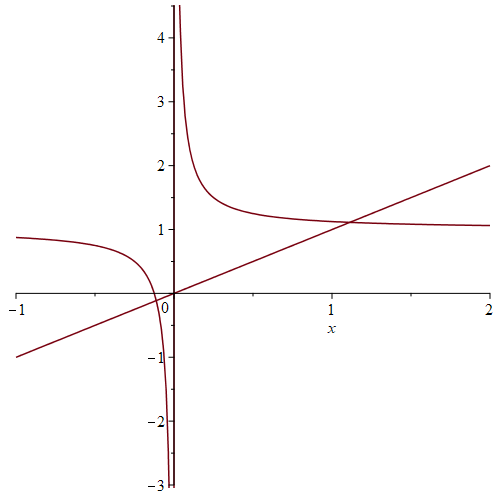
\includegraphics[scale=0.4]{1_2_fixedPoints.png}
		\end{minipage}
	\hfill
		\begin{minipage}{0.2\textwidth}
			$a=4,\\b=0.5,\\ c=4,\\ d=0\\$
		\end{minipage}
	\caption{Two fixed points on a Mobius function}
	\label{fig:mobFix}
	\end{figure}
\newpage
\subsubsection{The case for single fixed points}\label{ss_sfix}
Single fixed points occur exactly when $(d-a)^2+4bc=0$, as this only produces one real solution for the quadratic $cx^2+x(d-a)-b=0$, our fixed point condition. An example of this can be seen with the following Mobius parameters;
	\[a=3,\;b=-2,\;c=0.5,\;d=1,\;x_0=10\]
Plainly, the Mobius function will only touch the line $y=x$ in one position\footnote{And is therefore tangent to $y=x$} and thus only gives our function one fixed solution. We can see the values of the iterates in the table below, or on Figure \ref{fig:mobConvs}
	\begin{table}[h]
		\begin{center}
			\begin{tabular}{|c|c|}
				\hline
				 $n$  &    $x_n$     \\ \hline\hline
				  0   & 10.000000000 \\ \hline
				  1   & 4.666666667  \\ \hline
				  2   & 3.599999999  \\ \hline
				  3   & 3.142857143  \\ \hline
				  4   & 2.888888888  \\ \hline
				  5   & 2.727272727  \\ \hline
				\dots &    \dots     \\ \hline
				 20   & 2.205128205  \\ \hline
				 21   & 2.195121952  \\ \hline
			\end{tabular}
		\end{center}
	\end{table} \\
It is simple to deduce that with each iterate, $i$, the value of $x_i$ approaches a value. We can assume this is the value of the single fixed point of the graph although it is easy to check by performing the following;
		\begin{equation*}
			\begin{split}
				x&=\frac{ax+b}{cx+d} \\[5pt]
				cx^2+dx&=ax+b \\[5pt]
				0&=cx^2+x(d-a)-b \\[5pt]
				&=0.5x^2-2x+2\\[5pt]
				x&=\frac{-(d-a)\pm\sqrt{(d-a)^2+4cb}}{2c}\\[5pt]
				&=\frac{2\pm0}{1}\\[5pt]
				x&=2
			\end{split}
		\end{equation*}
Given that the fixed $x$ point is now known to be $x_{\mathrm{fix}}=2$, it seems reasonable to suggest that this is the value that the sequence above is converging towards.
	\begin{figure}[H]
		\centerline{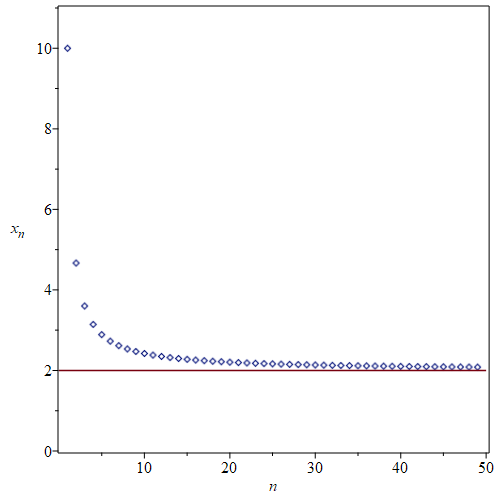
\includegraphics[scale=0.4]{mobFixConv.png}}
		\caption{A better way to visualise the convergence of the sequence towards a fixed point, plotting $x_n$ against $n$}
		\label{fig:mobConvs}
	\end{figure} \noindent
As this is the point where $f(x)=x$, the gradient at this repeated fixed point will always have a value of 1 as it is tangent to the line $y=x$
This can be shown to occur in all Mobius sequences with one fixed point -- the sequence will converge towards the value of the fixed point. The only exception to this occurs when $x_0$ is set to the $x$-value of the fixed point. In that case, the sequence will remain constant as there is no other fixed point to converge towards. \\
In the case that the discriminant is greater than 0, there will be more than one solution to the fixed point equation. In the next section we will explore how the sequence behaves in this case.
\subsubsection{The case for multiple fixed points}
In the case that there is more than one solution for the fixed points equation, there will be more than one fixed point also. This presents a problem as previously we would have expected the fixed point to be an attracting point to which the sequence converges. However, with two fixed points there is the question of which fixed point the sequence is attracted towards. Looking at examples, we can see through inspection that the attracting point of the sequence is that which has the least gradient.
It can be shown also that the gradients of the two fixed points have the following property;
\begin{gather*}
\abs[\Big]{\frac{\mathrm{d}f}{\mathrm{d}x}|_{x=\alpha}}<1<\abs[\Big]{\frac{\mathrm{d}f}{\mathrm{d}x}|_{x=\beta}} \\
\text{\footnotesize{where $\alpha$ and $\beta$ are the roots of $cx^{2}+x(d-a)-b$}} \\
\intertext{This property can be shown to simplify nicely to}
\abs[\Big]{\frac{\mathrm{d}f}{\mathrm{d}x}|_{x=\alpha}}\abs[\Big]{\frac{\mathrm{d}f}{\mathrm{d}x}|_{x=\beta}}=1
\end{gather*}
As the attracting fixed point is always the one with the lesser gradient, it follows that $\abs[\Big]{\frac{\mathrm{d}f}{\mathrm{d}x}|_{x=\gamma}}\le1$ for fixed point $\gamma$ for it to be attractive. \\
Questions are raised when there are no real solutions to $cx^{2}+x(d-a)-b$ and therefore no fixed points for $f(x)$. In \S\ref{sec:mobCycles} we will explore what happens to the Möbius sequence in the case of non-convergence towards a fixed point.
\subsection{Cobweb diagrams}\label{sec:cobs}
Cobweb diagrams are a way to view the iterations of a sequence in order to see how it develops as we progess towards the $n$\textsuperscript{th} iterate of a sequence. We can use this to our advantage to see the values of the Möbius sequence tending towards the attracting fixed points that are present. Taking the example below, we can see that the sequence converges towards the fixed point in a flip-flop fashion, never truly hitting the fixed point. The values of the iterates are represented on the cobweb diagram as an intersection on the line $y=x$, with the co-ordinate $\left[x_n,\;x_n\right]$
	\begin{figure}[H]
		\begin{minipage}{0.725\textwidth}
			\hfill
			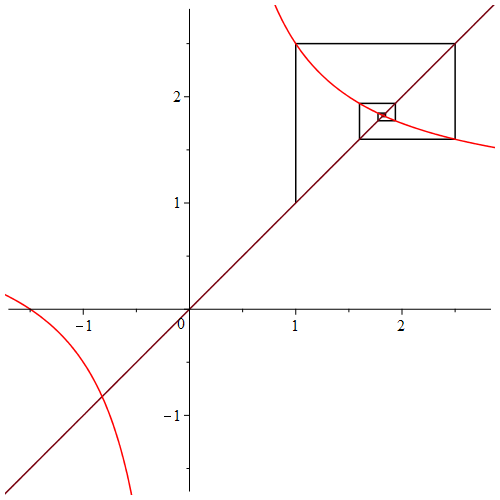
\includegraphics[scale=0.4]{fixedPointsCobwebIg.png}
		\end{minipage}
	\hfill
		\begin{minipage}{0.2\textwidth}
			$a=2,\\b=3,\\ c=2,\\ d=0\\$
		\end{minipage}
	\caption{Cobweb plot showing convergence towards a fixed point on a Möbius function}
	\label{fig:mobAp}
	\end{figure}
We can also see the way in which the sequence will always tend towards the attracting fixed point no matter how close to the repelling fixed point $x_0$ is in the figure below, which is the same graph with the other fixed point left exposed and $x_0=-0.8$.
We can also verify that the sequence will always converge to the attracting fixed point, no matter how close to the non-attracting fixed point.
	\begin{figure}[H]
		\begin{minipage}{0.725\textwidth}
			\hfill
			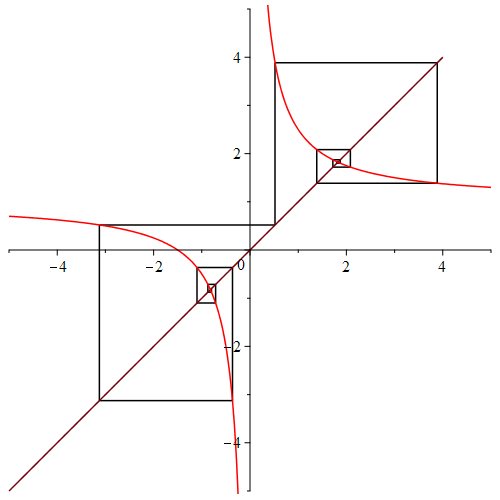
\includegraphics[scale=0.4]{fixedPointsCobwebMinOne.png}
		\end{minipage}
	\hfill
		\begin{minipage}{0.2\textwidth}
			$a=2,\\b=3,\\ c=2,\\ d=0\\x_0=-0.8$
		\end{minipage}
	\caption{Convergence towards attracting fixed point when $x_0$ is close to the repelling fixed point}
	\label{fig:mobAs}
	\end{figure}
\subsection{Conditions for an $n$-cycle Möbius sequence}\label{sec:mobCycles}
The first case with non-fixed points that is of interest is when we choose specific values of $a, b, c$ or $d$ such that we may come across a sequence in which the terms repeat after $n$ iterations. I will be referring to these as $n$-cycle sequences. An example for a $3$-cycle can be seen using the variables 
	\[a=1,\; b=-\sqrt{3},\; c=\sqrt{3},\; d=1\]
which produces the following output:
	\[1,\; \frac{1-\sqrt{3}}{1+\sqrt{3}},\; \frac{-1-\sqrt{3}}{\sqrt{3}-1},\; 1,\; \frac{1-\sqrt{3}}{1+\sqrt{3}},\; \frac{-1-\sqrt{3}}{\sqrt{3}-1},\; \dots\]\label{seqout}
We can attempt to work out the condition of $a, b, c$ and $d$ that allow this $3$-cycle to occur by solving $f^3(x)$ symbolically\footnote{In this report, $f^n(x)$ refers to repeated iterations of $f$ as opposed to $n$\textsuperscript{th} derivatives of $f$}. The condition for a $3$-cycle is such that 
	\begin{equation*}
		\begin{split}
			f^3(x)   & =x \\[5pt]
			f^3(x)-x & =0
		\end{split}
	\end{equation*} 
Solving this gives us 
	\begin{equation*}
		\begin{split}
			f^3(x)-x & =\frac{(a^2+ad+bc+d^2)(-cx^2+x(a-d)+b)}{bc^2x+c(x(a^2+ad+d^2)+b(a+2d))+d^3} \\[5pt]
			0        & =\frac{(a^2+ad+bc+d^2)(-cx^2+x(a-d)+b)}{bc^2x+c(x(a^2+ad+d^2)+b(a+2d))+d^3} \\[5pt]
			         & =(a^2+ad+bc+d^2)(-cx^2+x(a-d)+b)
		\end{split}
	\end{equation*}
From this, we can see that either the first or second bracket has to equal zero in order for this condition to hold true. The condition that depends on $x$ shows us that there are certain values of $x$ that are fixed points, as shown previously. But as we would like a condition that is invariant of $x$ we will set the first bracket equal to zero in order to get our condition for a 3-cycle as
	\[a^2+ad+bc+d^2=0\]
Which, as expected, satisfies our values for $a, b, c$ and $d$.
We can use this method to find other conditions for other cycle lengths also. The table below outlines the conditions for cycle lengths 2 through 6;
	\begin{table}[H]
		\begin{center}
			\begin{tabular}{|c|c|}
				\hline
				Cycle Length &                           True Condition                           \\ \hline\hline
				     2       &                              $a+d=0$                               \\ \hline
				     3       &                         $a^2+ad+bc+d^2=0$                          \\ \hline
				     4       &                          $a^2+2bc+d^2=0$                           \\ \hline
				     5       & $b^2c^2+3bc(a^2 + \frac{4}{3}ad + d^2)+a^4+a^3d+a^2d^2+ad^3+d^4=0$ \\ \hline
				     6       &                         $a^2-ad+3bc+d^2=0$                         \\ \hline
			\end{tabular}
		\end{center}
	\end{table}
\noindent The reason for calling the second column True Condition is due to the fact that a cycle length of $n$ will contain the conditions for cycle lengths equal to its factors. For example, the condition for a cycle length of 4 contains both $a^2+2bc+d^2=0$ and $a+d=0$, the former being the true condition as it is not present in the conditions for a 2 cycle. 
However, this becomes a problem as we attempt to find conditions for higher $n$-cycles as the true conditions become of a higher order or they just become more complex in general. The conditions are most complex when $n$ is a prime number due to the fact that there are no conditions present from factors\footnote{Besides the factor 1, which gives us fixed points}. This is an issue when we try to generate examples of certain $n$-cycles as the conditions become harder to solve for a particular variable.
This obstacle is overcome later in this chapter, where we will eventually find a general equation for the variables $a,\;b$ and $d$ for any cycle length, $n$ -- along with a few strange observations.
\subsubsection{Cobweb diagrams to visualise cycles}
We can use the cobweb diagrams that we explored in \S\ref{sec:cobs} in order to help us visualise cycles in the Möbius sequence. This time, instead of showing us a convergence towards a fixed point, the cobweb will repeat itself, with the number of solutions on $y=x$ reflecting the cycle number of the Möbius sequence. 
	\begin{figure}[H]
		\begin{minipage}{0.725\textwidth}
			\hfill
			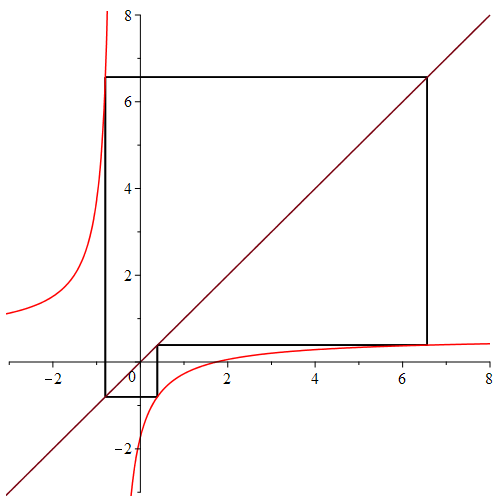
\includegraphics[scale=0.4]{mobCob3.png}
		\end{minipage}
	\hfill
		\begin{minipage}{0.2\textwidth}
			$a=1,\\b=-\sqrt{3},\\ c=\sqrt{3},\\ d=1\\$
		\end{minipage}
	\caption{Cobweb plot for a 3-cycle Möbius sequence}
	\label{fig:mobAsmp}
	\end{figure}
\noindent Here, we can see a cycle around the values obtained from the sequence in \S\ref{sec:mobCycles}. We can tell a cycle apart from other behaviours as the cobweb forms a \textbf{closed loop} around the iterates that give the $n$-cycle
\newpage
\subsection{Matrices as a representation of the Möbius sequence}
We can take our Mobius function and model it as a matrix, $M$, instead.
\[M=\begin{bmatrix}
	a & b \\
	c & d
\end{bmatrix}\]
For some $n$-cycle, the resulting final matrix will be found in the following way
\[M^n \begin{bmatrix} x_0 \\ 1 \end{bmatrix} = k \begin{bmatrix} x_n \\ 1 \end{bmatrix}\]
Considering that $x_0$ is apart of an $n$-cycle, $x_0$=$x_n$
\[M^n \begin{bmatrix} x_0 \\ 1 \end{bmatrix} = k \begin{bmatrix} x_o \\ 1 \end{bmatrix}\]
Letting $M^n$ take the form
\[M^n = \begin{bmatrix} \alpha & \beta \\ \mu & \nu \end{bmatrix}\]
By relying on the fact that this holds for all values of $x_0$, it follows that
\[\begin{bmatrix} \alpha & \beta \\ \mu & \nu \end{bmatrix}\begin{bmatrix} x_0 \\ 1 \end{bmatrix}=\begin{bmatrix} kx_0 \\ k \end{bmatrix}\]
\begin{align*}
	\alpha x_0+\beta & =kx_0                \\
	\mu x_0+\nu      & = k                  \\
	\alpha x_0+\beta & =x_0(\mu x_0+\nu)    \\
	                 & =\mu {x_0}^2+\nu x_0
\end{align*}
\begin{alignat*}{3}
	x_0 & =-1 & \quad\Longrightarrow\quad &  & \beta   & = 0       \\
	x_0 & =0  & \quad\Longrightarrow\quad &  & \alpha  & = \mu+\nu \\
	x_0 & =1  & \quad\Longrightarrow\quad &  & -\alpha & = \mu-\nu \\
	x_0 & =2  & \quad\Longrightarrow\quad &  & 2\alpha & = 2\nu
\end{alignat*}
From this system of equations, we can deduce that
\begin{align*}
	\beta  & =0   \\
	\mu    & =0   \\
	\alpha & =\nu
\end{align*}
And that by swapping this for the $M^n$ that we had before;
\begin{align*}
M^n &= \begin{bmatrix}
	\alpha & 0      \\
	0      & \alpha
\end{bmatrix} \\
	&= \alpha I
\end{align*}

\newpage
This must mean that for the matrix to represent a Möbius sequence with a fixed cycle length of $n$, there must be some power of the matrix that becomes a scalar matrix. Infact, the smallest value of $n$ for which $M^n$ is scalar is what gives us the length of the cycle.
\subsubsection{Application to eigenvalues of matrices}\label{sec:mobEig}
%%%%%%%%%%%%%%% 
We can progress further into the cyclic nature of some Möbius sequences by investigating in particular the ratio of the eigenvalues when representing the Möbius function as a matrix such that $M = \begin{bmatrix} a & b \\ c & d \end{bmatrix}$
with its eigenvalues, $\lambda_1$ and $\lambda_2$ derived from 
$\begin{vmatrix}
	a-\lambda & b         \\
	c         & d-\lambda
\end{vmatrix} = 0$ giving a quadratic for the values of $\lambda$ as follows
		\begin{align*}
			\begin{vmatrix}
				a-\lambda & b         \\
				c         & d-\lambda
			\end{vmatrix} &= 0 \\[5pt]
			(a-\lambda)(d-\lambda)-bc&=0 \\[5pt]
			{\lambda}^2-\lambda(a+d)+ad-bc&=0
		\end{align*}

And solving for $\lambda$ we can see that
	\[\lambda=\frac{a+d\pm\sqrt{(a+d)^2-4(ad-bc)}}{2}\]
\\ \noindent Using the known 3 cycle from \S\ref{sec:mobCycles} we can find the eigenvalues for the corresponding \textbf{`Möbius matrix'} by simplify substituting them into the eigenvalues equation above. For example, 
	\begin{equation*}
		\begin{split}
			\lambda & =\frac{2\pm\sqrt{-12}}{2} \\
			        & =1\pm\sqrt{3}i
		\end{split}
	\end{equation*}
The ratio of these eigenvalues can be seen as 
	\[\frac{\lambda_1}{\lambda_2}=\frac{1+\sqrt{3}i}{1-\sqrt{3}i}\]
Taking the powers of this ratio gives us the following
	\begin{equation*}
		\begin{split}
			\frac{\lambda_1}{\lambda_2}                & =-\frac{1}{2}+\frac{\sqrt{3}i}{2} \\[10pt]
			\left(\frac{\lambda_1}{\lambda_2}\right)^2 & =-\frac{1}{2}-\frac{\sqrt{3}i}{2} \\[10pt]
			\left(\frac{\lambda_1}{\lambda_2}\right)^3 & =1                                \\[10pt]
			\left(\frac{\lambda_1}{\lambda_2}\right)^4 & =-\frac{1}{2}+\frac{\sqrt{3}i}{2}
		\end{split}
	\end{equation*}
Which continues in this way such that
	\[\left(\frac{\lambda_1}{\lambda_2}\right)^{n+3}=\left(\frac{\lambda_1}{\lambda_2}\right)^n\]
Using the fact that the ratio of eigenvalues for $a,\;b,\;c,\;d\in\ \mathbb{R}$ always has modulus 1, we can visualise the successive powers of the ratio as rotations on the unit circle like so
	\begin{figure}[H]
		\centerline{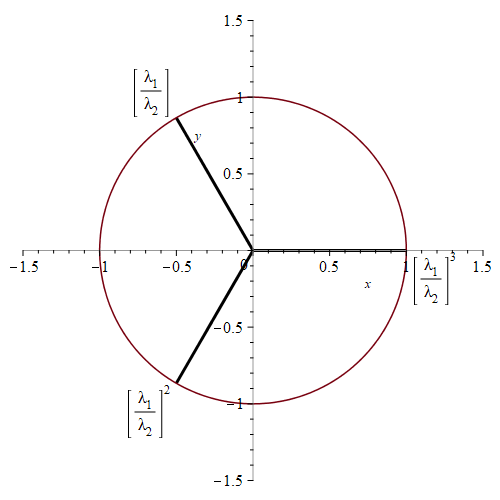
\includegraphics[scale=0.4]{eigenCycle.png}}
		\caption{Representing $n$\textsuperscript{th} roots of unity on an Argand diagram}
	\label{fig:eigenCycle}
	\end{figure}
If this is true, then the ratio of eigenvalues is said to be an $n$\textsuperscript{th} root of unity. A primitive $n$\textsuperscript{th} root of unity has the property that
\begin{align*}
	\left(\frac{\lambda_1}{\lambda_2}\right)^n&=1 \\
	\left(\frac{\lambda_1}{\lambda_2}\right)^k&\neq1 \\
	\intertext{for some $k=\left\{k:0<k<n,\;\left(k,n\right)\in\mathbb{Z}\right\}$}
\end{align*}
\newpage
\subsection{Generalisation \& the choice to remove the $c$ variable}\label{sec:mobGen}
It is possible to also reduce the number of variables that we need to consider -- this will make it easier to then try to produce a general equation to encompass all cycle lengths.
Consider first;
\begin{align*}
	f(x) & = \frac{ax+b}{cx+d} \\ \intertext{Considering first that $c=0$, we get the following;}
	f(x) & = \frac{ax+b}{d}    \\ \intertext{This is an uninteresting case in terms of Mobius sequences, as this funciton is now constant and will produce a linear sequence. Considering instead that $c=1$;}
	f(x) & = \frac{ax+b}{x+d}  \\ \intertext{This is not constant for all $x_0$ -- a propertry which we want. We can therefore treat all cases considering $c=1$. This narrows our choice for variables but makes it easier to generalise the equation}
\end{align*}
With this, we can plot equations for the cycles of a Möbius sequence by parametrising a variable such as $b$ in the true cycle conditions. For example, the possible values for $a\;,b$ and $d$ in a 3-cycle can be represented by the surface given by the co-ordinates
\[\left\{a,\quad -a^2-ad-d^2,\quad d\right\}\]
Other possible cycles can be visualised in a similar fashion. Although it does again become more difficult for higher order cycle conditions, where even removing the $c$ variable is not enough to parametrise for a variable. This obstacle is surpassed in \S\ref{sec:mobGenEq}, where we explore how to form a general equation for all cycle lengths. The table below outlines the co-ordinate surfaces that represent a cycle length of $n$ for cycle lengths 2 to 6
	\begin{table}[H]
		\begin{center}
			\begin{tabular}{|c|c|}
				\hline
				$n$ &          Co-ordinate surface          \\[4pt] \hline\hline
				 2  &    $\left\{a,\; 0,\; d \right\} $     \\[4pt] \hline
				 3  &      $\{a,\; -a^2-ad-d^2,\; d\}$      \\[4pt] \hline
				 4  &  $\{a,\;\frac{-a^2-d^2}{2},\; d\} $   \\[4pt] \hline
				 5  & This is too complex to solve for $b$  \\[4pt] \hline
				 6  & $\{a,\;\frac{-a^2+ad-d^2}{3},\; d\} $ \\[4pt] \hline
			\end{tabular}
		\end{center}
	\end{table}
\newpage
\subsection{General equation for an $n$-cycle Möbius sequence}\label{sec:mobGenEq}
We can use what we have learned from \S\ref{sec:mobEig} and \S\ref{sec:mobGen} to produce a general equation that covers all possible $n$-cycles. This has many advantages over previous methods, the most being that we can now plot very high order cycles with ease.\\
We must first find the symbolic results for the sum and the product of the eigenvalues, and that can be done like so;

\begin{equation*}
	\begin{split}
		\lambda_1+\lambda_2               & =\frac{a+d+\sqrt{(a+d)^2-4(ad-bc)}}{2}+\frac{a+d-\sqrt{(a+d)^2-4(ad-bc)}}{2}                          \\
		                                  & =a+d                                                                                                  \\
		                                  &                                                                                                       \\
		\lambda_1\lambda_2                & =\left(\frac{a+d+\sqrt{(a+d)^2-4(ad-bc)}}{2}\right)\left(\frac{a+d-\sqrt{(a+d)^2-4(ad-bc)}}{2}\right) \\
		\text{Which simplifies nicely to} &                                                                                                       \\[10pt]
		\lambda_1\lambda_2                & =ad-bc
	\end{split}
\end{equation*}
We can use these facts as the basis of our general equation;, along with setting up our eigenvalues as follows (assuming $\lambda_1$ and $\lambda_2$ are eigenvalues of an $n$-cycling sequence)
	\begin{align*}
		\frac{\lambda_1}{\lambda_2}      & =\alpha                                                           \\[10pt]
		a+d                              & =\lambda_1+\lambda_2                                              \\
		                                 & =\lambda_2+\lambda_2\alpha                                        \\
		                                 & =\lambda_2\left(1+\alpha\right)                                   \\[10pt]
		\lambda_2                        & =\frac{a+d}{1+\alpha}                                             \\[10pt]
		ad-bc                            & =\lambda_1\lambda_2                                               \\
		                                 & =\alpha{\lambda_2}^2                                              \\
		                                 & =\alpha\left(\frac{a+d}{1+\alpha}\right)^2                        \\ \intertext{It follows that}
		\frac{\left(a+d\right)^2}{ad-bc} & =\frac{{\lambda_2}^2\left(1+\alpha\right)^2}{\alpha{\lambda_2}^2} \\[10pt]
		                                 & =\frac{\left(1+\alpha\right)^2}{\alpha}                           \\[10pt]
		                                 & =\alpha+\alpha^{-1}+2                                             \\ \intertext{As shown previously, $\alpha$ is of modulus one (due to the fact cycles lie on the unit circle) -- we can therefore deduce that}
		\frac{\left(a+d\right)^2}{ad-bc} & =2\left(1+\Re\left({\alpha}\right)\right)
	\end{align*}
Where $\Re\left(\alpha\right)$ is the real part of $\alpha$.\\ \\
Similarly as to before, we can also choose to remove the $c$ variable with little to no loss to generality, and that then gives us an equation for $a, b \text{ \& } d$ in terms of $\alpha$
\[\left(a+d\right)^2=2\left(1+\Re\left(\alpha\right)\right)\left(ad-b\right) \text{	where	}\alpha=\cos\left(\frac{2k\pi}{n}\right)+i\sin\left(\frac{2k\pi}{n}\right)\]
With this equation, we can now choose cycle lengths of $n$, where $k,\ n$ share no common factors. For example, the seven cycle parameters for $a, b, d$ are given by
	\begin{align*}
		\left(a+d\right)^2 & =2\left(1+\Re\left(\frac{2k\pi}{7}\right)\right)\left(ad-b\right)               \\
		                   & \text{\footnotesize{\;\;\;	where	}}{\scriptstyle k=1,\ 2,\ 3}                   \\ \intertext{Armed with this new method of finding cycles in a Möbius sequence, we can attempt to construct surfaces in $a,\ b,\ d$ space by parametrising the variable $b$ as follows.}
		\left(a+d\right)^2 & =2\left(1+\Re\left(\frac{2k\pi}{7}\right)\right)\left(ad-b\right)               \\
		ad-b               & =\frac{\left(a+d\right)^2}{2\left(1+\Re\left(\cfrac{2k\pi}{7}\right)\right)}    \\
		b                  & =ad-\frac{\left(a+d\right)^2}{2\left(1+\Re\left(\cfrac{2k\pi}{7}\right)\right)} \\
		                   & \text{\footnotesize{\;\;\;	where	}}{\scriptstyle k=1,\ 2,\ 3}
	\end{align*}
Using this, we can plot with respective values of $k$ in a graphing package such as the \texttt{plot3d} command in Maple using the co-ordinates below in $a,\;b,\;d$ space. Infact, this can be used for all cycle lengths by giving different values of $n$.
\[\left[a,\;ad-\frac{\left(a+d\right)^2}{2\left(1+\Re\left(\cfrac{2k\pi}{7}\right)\right)},\;d\right]\]
Using the 7-cycle Möbius sequence as an example, we get 3 different surfaces for the 3 different values of $k$ that look like this in $a,\;b,\;d$ space.
\begin{figure}[H]
	\centering
	\begin{minipage}{.3\textwidth}
		\centering
		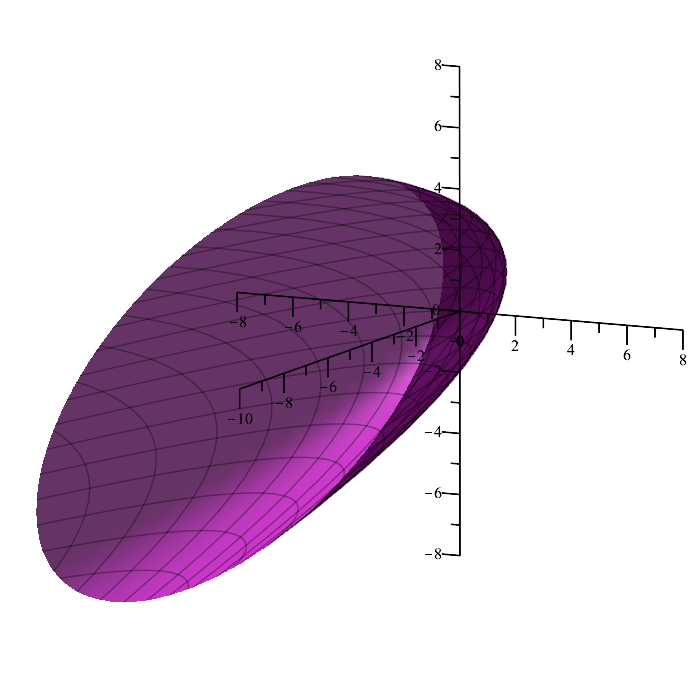
\includegraphics[width=\linewidth]{mob7Cyc2.png}
		\captionof{figure}{7-cycle for $k=1$}
		\label{fig:test1}
	\end{minipage}%
	\begin{minipage}{.3\textwidth}
		\centering
		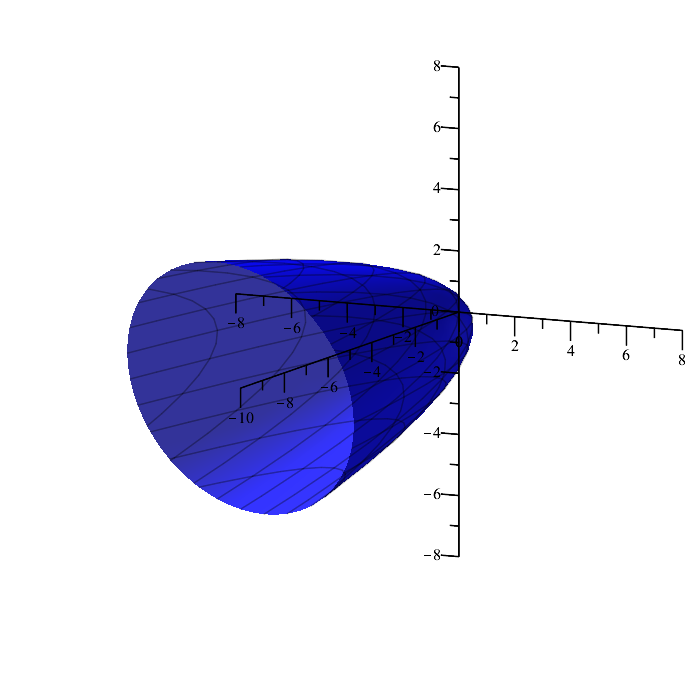
\includegraphics[width=\linewidth]{mob7Cyc4.png}
		\captionof{figure}{7-cycle for $k=2$}
		\label{fig:test1}
	\end{minipage}%
	\begin{minipage}{.3\textwidth}
		\centering
		\includegraphics[width=\linewidth]{mob7cyc6.png}
		\captionof{figure}{7-cycle for $k=3$}
		\label{fig:test2}
	\end{minipage}
\end{figure}
\noindent Rather interestingly, when placed all on the same plot the different paraboloids stack inside each-other - touching along the same two curves. We can easily see this in the plot below.
\begin{figure}[H]
	\centering
	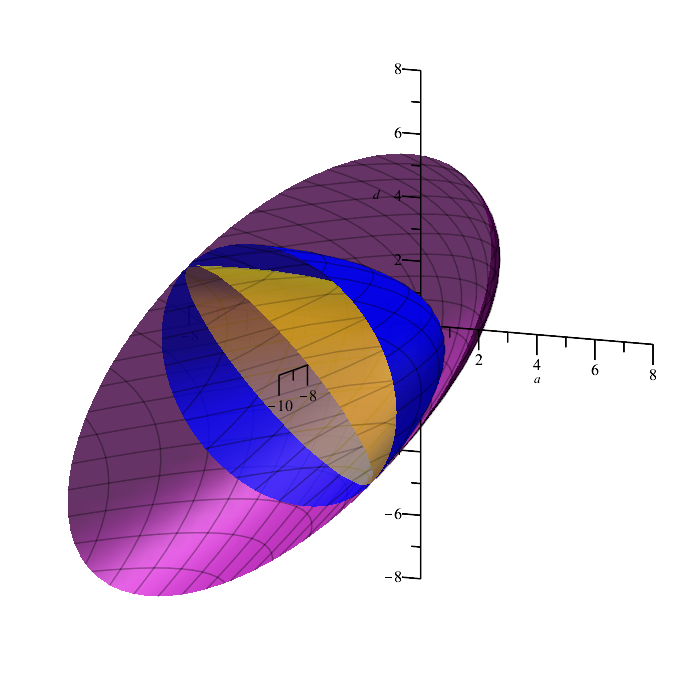
\includegraphics[scale=0.3]{mob7Cyc.png}
	\caption{All 7-cycles plotted in the same $a,\;b,\;d$ space}
\end{figure}
Perhaps the most surprising thing is that there are multiple surfaces that give the $a,\;b,\;d$ variables for a particular cycle length\footnote{This is not true for $n=0,\;1,\;2$}. In fact, we can work out the number of surfaces that a given cycle has using the Euler totient function\footnote{A thorough definition is provided in the appendix} with the notation
	\[\phi(n)\]
The totient function is defined as ``the number of positive integers $\le n$ that are relatively prime to $n$, i.e.\ they do not contain any factor in common with $n$''\cite{totient}. One is defined as relatively prime to all numbers. We need to then only take half of this number, due to the fact that the complex roots of unity come in conjugate pairs -- therefore, the sum of the pairs cancels out the imaginary parts and doubles the real part. 
\\
This works due to the fact that the condition on which the ratio of eigenvalues to some power equals 1 relies heavily on the fact that for $\alpha$ to be a primitive $n$\textsuperscript{th} root of one, $\alpha$ must lie on the unit circle and from that, some real rotation as a result of raising the ratio of eigenvalues to some $k\in\mathbb{Z} $ must return the result one.\\ \\
For a cycle of length $n$ we must therefore consider that there will be $\frac{\phi(n)}{2}$ branches of rotations on the unit circle. Therefore, we need to only consider $k$ for which there are no ways to reduce the denominator less than the intended cycle length of $n$, and for which $2k<n$. We can use this and find that all the real parts of $\alpha$ will be in the form
	\[\frac{2k\pi}{n}\]
\newpage
\section{The Period Doubling Sequence}\label{s_per}
The period doubling sequence comes from the quadratic $f(x)=rx(1-x)$  and its recurrence equation $x_{n+1}=rx_n(1-x_n)$ . The parameter $r$ can be perceived to change the `steepness' of the graph, with greater values of $r$ producing a steeper graph than lower values of $r$. An example of the graph can be seen below with $y=x$ overlayed also. In this section, $x_0=0.5$ unless otherwise stated.
	\begin{figure}[H]
		\begin{minipage}{0.725\textwidth}
			\hfill
			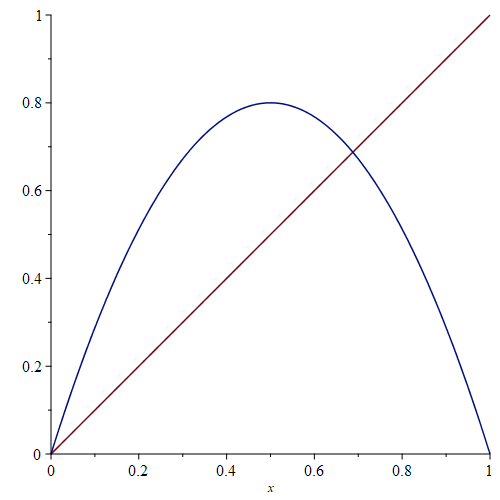
\includegraphics[scale=0.4]{periodExample.png}
		\end{minipage}
	\hfill
		\begin{minipage}{0.2\textwidth}
			$r=3.2$
		\end{minipage}
	\caption{$rx(1-x)$ against $y=x$}
	\label{fig:mobAsl}
	\end{figure}
It is easy to work out the $x$ values of the fixed points of this graph. That is, where
	\begin{equation*}
		\begin{aligned}
			f(x)       & =x \\
			rx(1-x)    & =x \\
			rx(1-x)-x  & =0 \\
			-rx^2+rx-x & =0 \\
			-x(rx-r+1) & =0
		\end{aligned}
	\end{equation*}
Which gives us the solutions
\[x = \Big \{0, \frac{r-1}{r}\Big \}\]
In later sections, we will explore how choosing a starting point in the sequence that is not a solution to $-x(rx-r+1)=0$ affects the period doubling sequence - once again leading towards the idea of cycles but also the idea of chaotic regions.
\newpage
\subsection{The period doubling sequence when $r<3$}
When $r<3$, the sequence always tends towards the fixed point where the modulus of the gradient is less than one, as expected. We can see an example of the cobweb diagram below, where we can see a convergence from $x_0$ towards the second fixed point.
\begin{figure}[H]
	\centering
	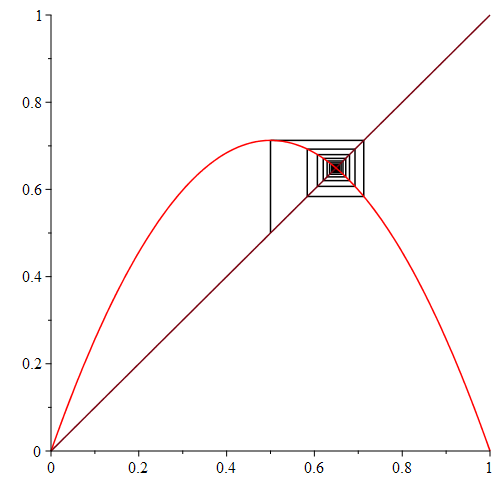
\includegraphics[scale=0.4]{perCob2p85.png}
	\caption{A cobweb plot showing convergence towards a fixed point on a period doubling sequence}
	\label{fig:percob2p85}
\end{figure}
This fixed point behaviour is the same as the fixed point behaviour on the Möbius sequence, which we would expect from any fixed point in general. One observation is that as $r\to3$ from below, the rate at which the sequence converges towards the fixed point decreases. This is due to the fact that as $r\to3$, the gradient of $f(x)$ at the attracting fixed point approaches -1. So whilst the successive iterations of the sequence may oscillate around the attracting fixed point, the difference between absolute value of the results starts to approach 0. For values very close to 3, the number of iterations needed to arrive at the fixed point starts to approach $\infty$. We can see an example of this on the following diagram, which plots the difference between the value of the attracting fixed point and $x_n$ against $n$ with different values of $r$
	\begin{figure}[H]
		\centering
		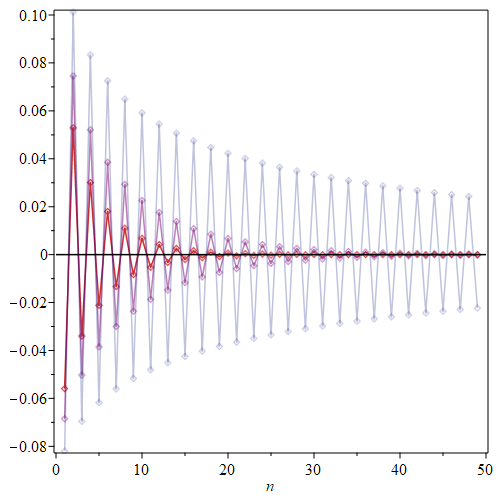
\includegraphics[width=10truecm, height=6truecm]{perDifferencesInR.png}
		\caption{\centering{A graph showing how different values of $r$ affects the rate of convergence $r=2.79,\;2.89,\;2.99$ from least transparent to most transparent respectively}}
		\label{fig:rateOfConvs}
	\end{figure}

\subsection{The period doubling sequence when $r\ge3$}
Considering $r>3$, we start to notice a different behaviour in the period doubling sequence. Whilst at first it looks as though the sequence converges towards the fixed point in a similar fashion to when $r<3$, that would be incorrect. Looking at a table of $x_n$ against the $n$\textsuperscript{th} iterate we can see that whilst it starts that way, there is an odd behaviour as $n$ gets sufficiently large.
	\begin{table}[H]
	\begin{center}
		\begin{tabular}{|c|c|}
			\hline
			 $n$  &    $x_n$    \\ \hline\hline
			  0   & 0.500000000 \\ \hline
			  1   & 0.762500000 \\ \hline
			  2   & 0.552335937 \\ \hline
			  3   & 0.754145896 \\ \hline
			  4   & 0.565500083 \\ \hline
			\dots &    \dots    \\ \hline
			1000  & 0.737704918 \\ \hline
			1001  & 0.590163934 \\ \hline
			1002  & 0.737704918 \\ \hline
			1003  & 0.590163934 \\ \hline
		\end{tabular}
	\end{center}
\end{table}
As we can see, instead of converging towards a fixed point the sequence has now converged towards a 2-cycle sequence. I will be referring to all period doubling sequences that follow this behaviour as limiting $n$-cycle sequences.
It is easier to see this on a diagram similar to Figure \ref{fig:rateOfConvs}, the only difference being plotting $x_n$ against $n$ this time. This can also be seen on a cobweb diagram in a similar way, so both are shown below
	\begin{figure}[H]
	\centering
	\hfill
	\begin{minipage}{.45\textwidth}
		\centering
		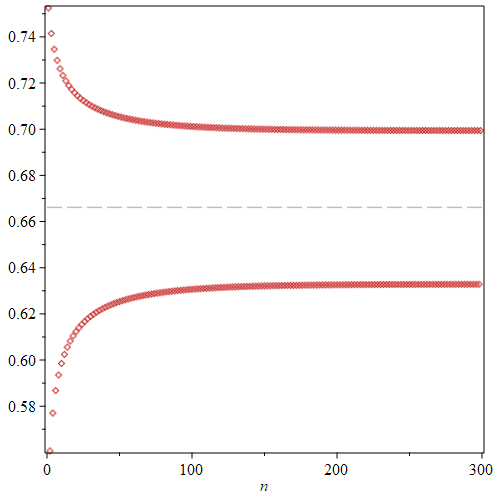
\includegraphics[scale=0.4]{per3p05Conv.png}
		\captionof{figure}{Converge towards a limiting 2-cycle in the period doubling sequence, plotting values of $x_n$}
		\label{fig:test1}
	\end{minipage}%
	\hfill
	\begin{minipage}{.45\textwidth}
		\centering
		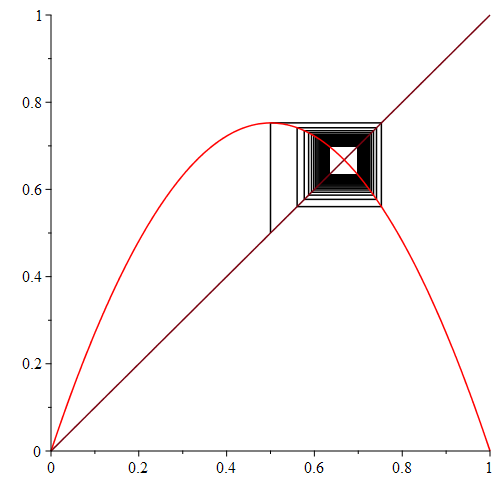
\includegraphics[scale=0.4]{per3p05Cob.png}
		\captionof{figure}{Converge towards a limiting 2-cycle in the period doubling sequence on a cobweb plot}
		\label{fig:test1}
	\end{minipage}%
	\hfill
	\end{figure}
\newpage
We can easily find the exact value of $x_0$ that gives a limiting 2-cycle by solving $f^2(x)-x=0$ for $x$, giving us the solutions
\[x=\left\{0,\;\frac{r-1}{r},\;\frac{\cfrac{r}{2}+\cfrac{1}{2}+\cfrac{\sqrt{r^2-2r-3}}{2}}{r},\;\frac{\cfrac{r}{2}+\cfrac{1}{2}-\cfrac{\sqrt{r^2-2r-3}}{2}}{r}\right\}\]
The first two solutions are already known to be for the fixed point of $f^2(x)$, we can therefore assume that the other two solutions are for the two starting values, left and right of the fixed point, that give a perfect 2-cycle (as opposed to a limiting 2-cycle)
Solving these for $r=3.01$, we get the solutions $x_0=\left\{0.6677740864,\;0.6993770505\right\}$.\\ 
As expected, choosing one of these starting values for the sequence gives us the following two plots, showing that this is a perfect 2-cycle.
\begin{figure}[H]
	\centering
	\hfill
	\begin{minipage}{.45\textwidth}
		\centering
		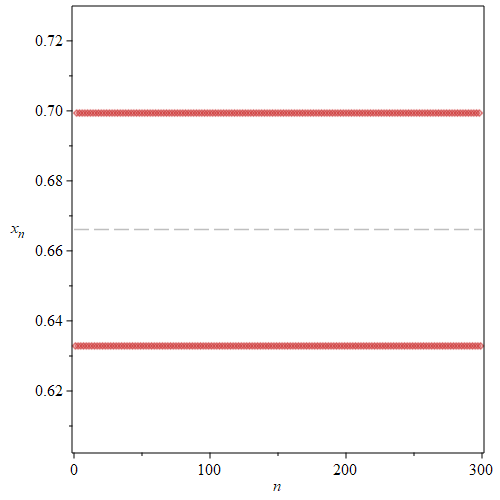
\includegraphics[scale=0.4]{per3p05Per.png}
		\captionof{figure}{Perfect 2-cycle on the period doubling sequence, plotting $x_n$ against $n$}
		\label{fig:test1}
	\end{minipage}%
	\hfill
	\begin{minipage}{.45\textwidth}
		\centering
		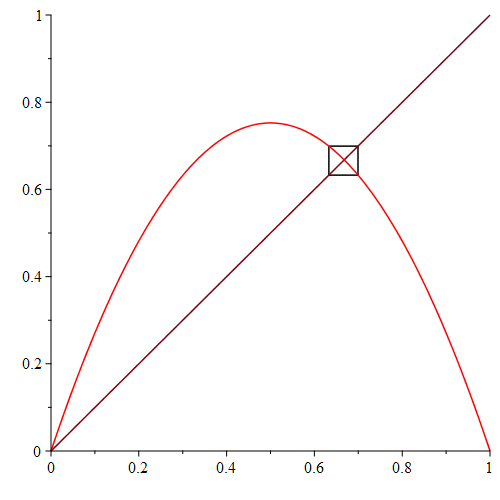
\includegraphics[scale=0.4]{per3p05PerCob.png}
		\captionof{figure}{Perfect 2-cycle on the period doubling sequence, shown via a cobweb plot}
		\label{fig:test1}
	\end{minipage}%
	\hfill
\end{figure}
This behaviour does not continue indefinitely however, with $r=3.5$ for example, the behaviour does not seem to be converging towards a 2-cyclel. In addition to this, choosing $x_0=0.8269407066$ produces the following plots;
\begin{figure}[H]
	\centering
	\hfill
	\begin{minipage}{.45\textwidth}
		\centering
		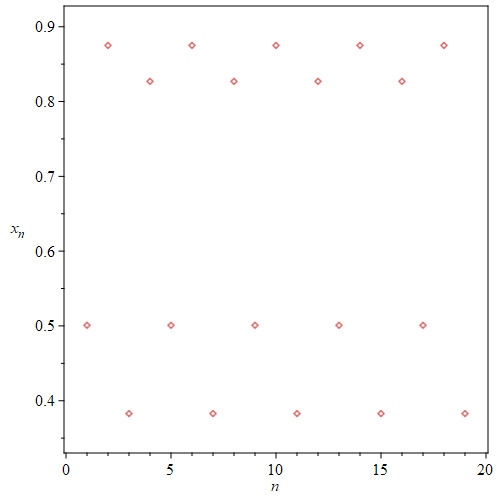
\includegraphics[scale=0.4]{per3p5Per.png}
		\captionof{figure}{Perfect 4-cycle on the period doubling sequence, plotting $x_n$ against $n$}
		\label{fig:test1}
	\end{minipage}%
	\hfill
	\begin{minipage}{.45\textwidth}
		\centering
		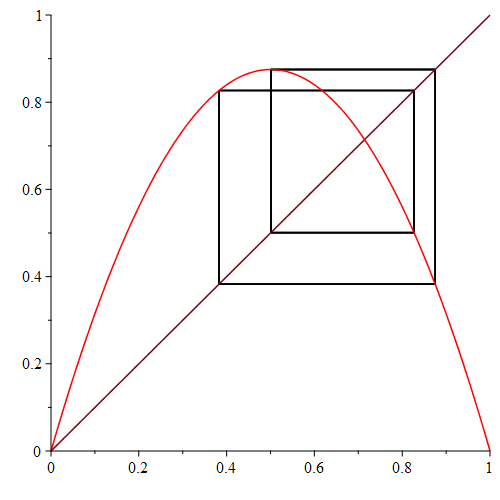
\includegraphics[scale=0.4]{per3p5PerCob.png}
		\captionof{figure}{Perfect 4-cycle on the period doubling sequence, shown via a cobweb plot}
		\label{fig:test1}
	\end{minipage}%
	\hfill
\end{figure}
From this, we can see that $r=3.5$ produces neither limiting nor perfect 2-cycles, it produces 4-cycle sequences instead. Increasing $r$ even further takes us to 8-cycles, then 16-cycles etc. until we hit the \textbf{chaotic} region of the period doubling sequence. There, we see no convergence towards cycles as $x_n$ seems to not follow any pattern at all. We can visualise this in the same way as previously ($r=3.8$);
\begin{figure}[H]
	\centering
	\hfill
	\begin{minipage}{.45\textwidth}
		\centering
		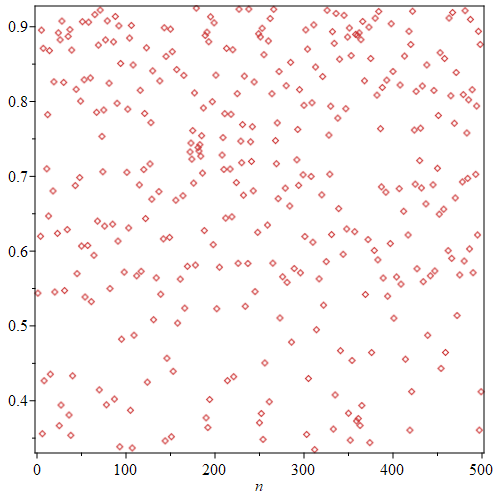
\includegraphics[scale=0.34]{per3p8.png}
		\captionof{figure}{Chaotic behaviour of the period doubling sequence, plotting $x_n$ against $n$}
		\label{fig:test1}
	\end{minipage}%
	\hfill
	\begin{minipage}{.45\textwidth}
		\centering
		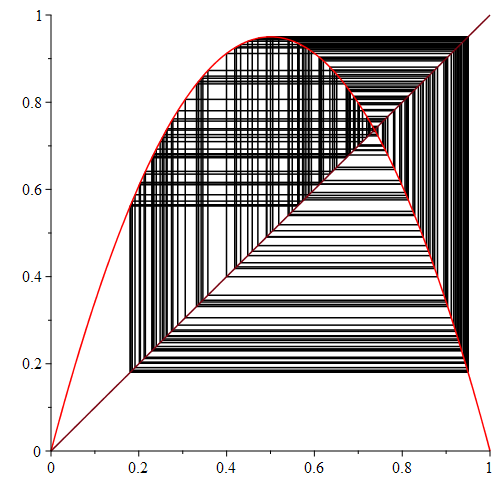
\includegraphics[scale=0.34]{per3p8Cob.png}
		\captionof{figure}{Chaotic behaviour of the period doubling sequence, shown on a cobweb plot}
		\label{fig:test1}
	\end{minipage}%
	\hfill
\end{figure}
As we can see, there does not seem to be any pattern to the values of $x_n$ -- all we have is a field of seemingly random points with no connection to one another, this is what we call \textbf{chaos} -- that is, small changes to the parameter $r$ yield dramatically different results to the output of the sequence
\newpage
\subsubsection{Finding the limit of $r$ for a limiting two cycle}
Since we know from previously that the value of the gradient for an attracting fixed point must be less than or equal to one (or else it repels), we can assume that by finding the $x$ co-ordinates that give a perfect two cycle in terms of $a$ and solving the condition that the differential of $f^2(x)\le1$ at these points, we will be able to find a range of values for $a$ in which a limiting two cycle occurs.
\\ \\
We start by solving $f^2(x)-x=0$ in terms of $r$ in order to get the point where an exact two cycle occurs - this will give us the same solutions as when we were finding the exact $x_0$ to give a two cycle. Using the 3\textsuperscript{rd} and 4\textsuperscript{th} solutions from Page 21 we can find the points in terms of $r$ which give a perfect 2-cycle. Whilst it is not immediately clear which one of these should be used, it can be shown that these two solutions produce the same gradient for all values\footnote{I believe this is due to the fact that these solutions are giving the exact two cycle around the fixed point, so the only difference is which side of the fixed point they lie on (due to the oscillating nature)} of $r$, so for our purpose I will stick with using the 4th solution (although it does not matter which we choose). \\
We then need to find the values of $a$ for which the condition below holds true.
\[\abs[\Big]{\frac{\mathrm{d}f\circ f}{\mathrm{d}x}}\le1\]
I will start by doing this graphically using both the \texttt{plot} and \texttt{implicitplot} packages from Maple
\begin{figure}[H]
	\centering
	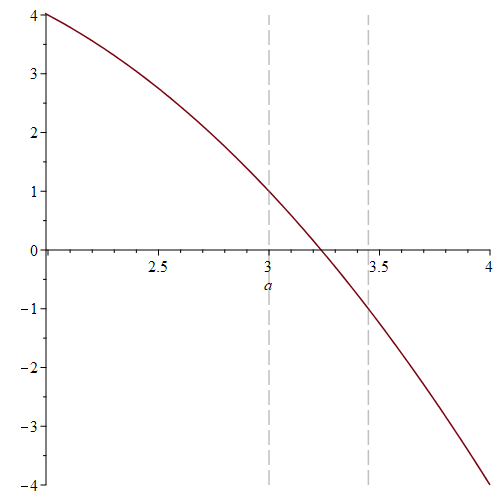
\includegraphics[scale=0.4]{1sqrt5lim.png}
	\caption{The values for the differential of $f^2(x)$ at one of the fixed points graphed against $a$}
\end{figure}
From this, we can see that there is a solution at $r=3$, as expected. This is due to the fact that the limiting 2-cycle behaviour starts at $r=3$. We can also see the other solution at $a\approx3.43$. After this value, there is no more two cycling of the period doubling sequence -- we can prove this by numerically checking the results of numbers around that area. It can also be solved for an exact value by using a package such as Maple.
\newpage
Although the calculation is much too long to include in this section of the report, the Maple code for calculating this upper limit will be in the appendix, the result of which gives the upper limit to be $1+\sqrt{6}$ (the negative answer has been ignored).
\\Although in theory this method would work to find any of the limits to the cycles, the application is rather different in practice; solving $f^n(x)$ for $n$ as little as 4 proves to be very difficult as a result of the degree of the polynomials that we are working with.
Packages such as Maple can solve these limits implicitly -- although this is at the loss of accuracy, especially when we get to higher cycle numbers as the distance between subsequent cycles decreases as the cycle number increases.
\subsection{Bifurcation diagrams}
``A Bifurcation Diagram is a visual summary of the succession of period-doubling produced as $r$ increases'' that is, plotting the values that a given $x_0$ approaches against the variable $r$. This sort of diagram helps us to visualise the period doubling sequence very easily.
\begin{figure}[H]
	\centering
	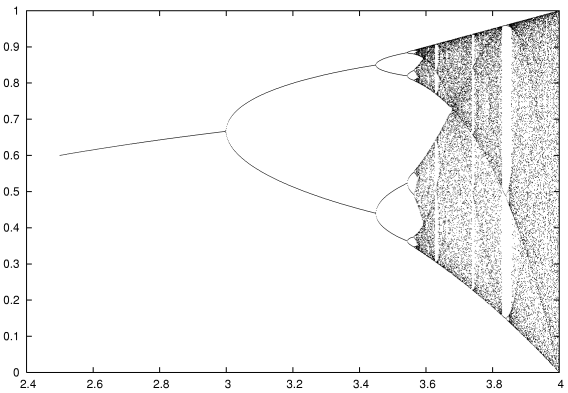
\includegraphics[scale=1.6]{bif.png}
	\caption{The bifurcation diagram of $rx\left(1-x\right)$ \; \cite{bifdia}}
	\label{fig:percob2p85}
\end{figure}
Here, we can see the start of the 2-cycling at $r=3$, and the end of the 2-cycling at $3.44949$ ($1+\sqrt{6}$). With $r$ between $3.44949$ and 3.54409 \cite{4cyclim, logis} we can see the 4-cycling occur, along with subsequent 8 and 16 cycles for higher values of $r$. When $r\gtrapprox3.56995$\cite{allcyclim, logis}, the period doubling sequence stars to behave chaotically in a \textbf{deterministic} fashion. This is different to randomness in that given the starting conditions, $x_0$ and $r$, we can \textbf{determine} what any value in the sequence will be -- randomness is \textbf{non-deterministic} in that even given all detail about the start of a system, the output can not be determined.
Another property more easily seen on the bifurcation diagram of $rx\left(1-x\right)$ is that the range of $r$ values that produce an $n$-cycle decreases as the cycle number, $n$, increases. This means that the choice of $r$ is restricted drastically when trying to find a 1024-cycle as opposed to an 8-cycle.
\subsection{Gaps in chaos}
Very strange cyclic behaviours can even be seen when $r$ has passed the chaotic threshold. These can be seen on the bifurcation diagram as `whitespace' among the field of black -- areas where the chaos falls back down into cyclic behaviour before then cascading back into chaos. Interestingly, we can observe cycles that are not powers of two. Some examples are below with $r=3.83169,\;3.738744,\;3.628389$ in order of appearance.
\newpage
\begin{figure}[H]
	\centering
	\hfill
	\begin{minipage}{.45\textwidth}
		\centering
		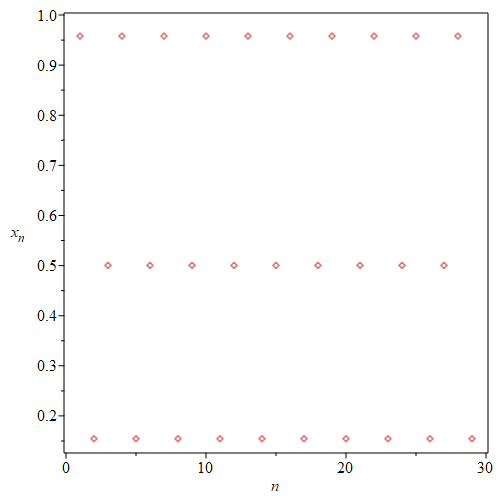
\includegraphics[scale=0.34]{per3p83169.png}
		\captionof{figure}{3 cycle in the chaotic region of the period doubling sequence, plotting $x_n$ against $n$}
		\label{fig:test1}
	\end{minipage}%
	\hfill
	\begin{minipage}{.45\textwidth}
		\centering
		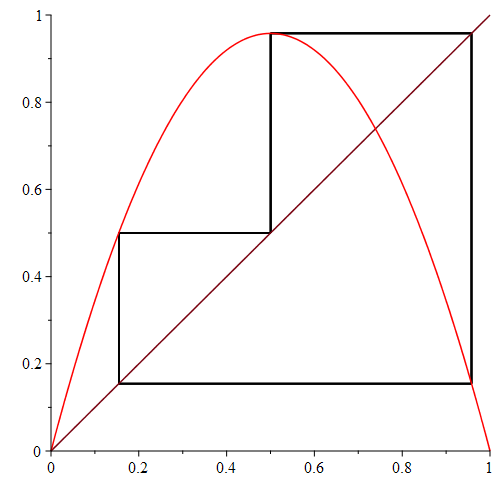
\includegraphics[scale=0.34]{per3p83169Cob.png}
		\captionof{figure}{3 cycle in the chaotic region of the period doubling sequence, shown on a cobweb plot}
		\label{fig:test1}
	\end{minipage}%
	\hfill
\end{figure}
\begin{figure}[H]
	\centering
	\hfill
	\begin{minipage}{.45\textwidth}
		\centering
		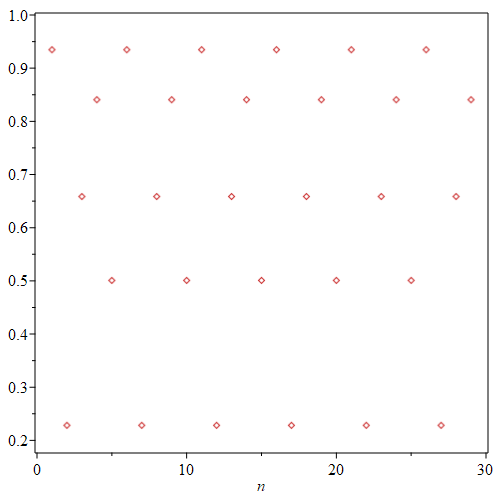
\includegraphics[scale=0.34]{per3p738744.png}
		\captionof{figure}{5 cycle in the chaotic region of the period doubling sequence, plotting $x_n$ against $n$}
		\label{fig:test1}
	\end{minipage}%
	\hfill
	\begin{minipage}{.45\textwidth}
		\centering
		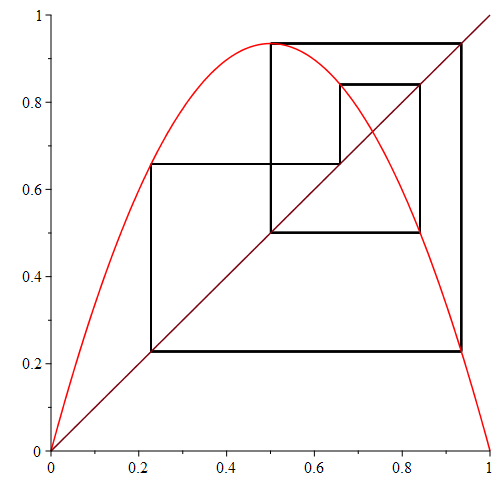
\includegraphics[scale=0.34]{per3p738744Cob.png}
		\captionof{figure}{5 cycle in the chaotic region of the period doubling sequence, shown on a cobweb plot}
		\label{fig:test1}
	\end{minipage}%
	\hfill
\end{figure}
\begin{figure}[H]
	\centering
	\hfill
	\begin{minipage}{.45\textwidth}
		\centering
		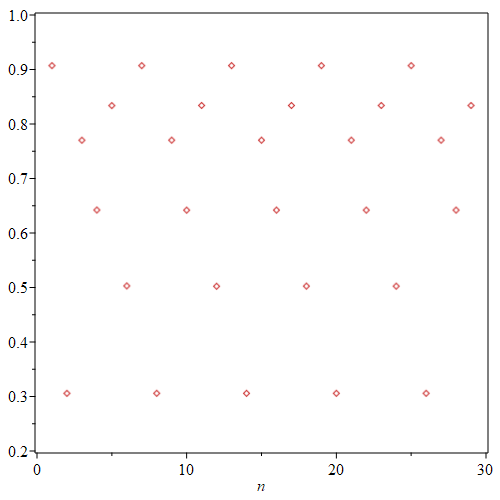
\includegraphics[scale=0.34]{per3p628389.png}
		\captionof{figure}{6 cycle in the chaotic region of the period doubling sequence, plotting $x_n$ against $n$}
		\label{fig:test1}
	\end{minipage}%
	\hfill
	\begin{minipage}{.45\textwidth}
		\centering
		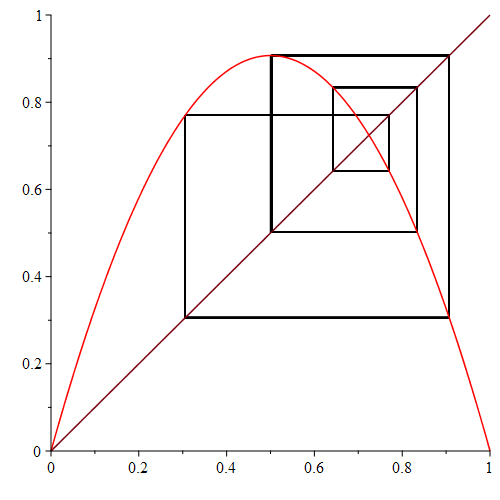
\includegraphics[scale=0.34]{per3p628389Cob.png}
		\captionof{figure}{6 cycle in the chaotic region of the period doubling sequence, shown on a cobweb plot}
		\label{fig:test1}
	\end{minipage}%
	\hfill
\end{figure}
\newpage
\subsection{The Butterfly Effect}
The Butterfly Effect refers to the sensitivity of the output with very small changes to initial conditions -- a property that defines chaos. 
\begin{figure}[H]
	\begin{minipage}{0.725\textwidth}
		\hfill
		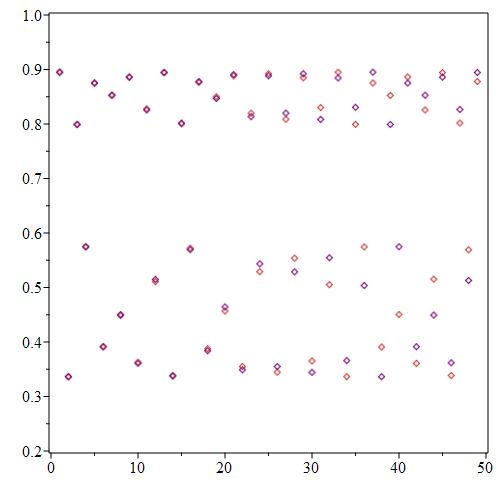
\includegraphics[scale=0.4]{butterfly.png}
	\end{minipage}
	\hfill
	\begin{minipage}{0.2\textwidth}
		\textcolor{orange}{$ r=0.500 $}\\\textcolor{Plum}{$ r=0.505 $}
	\end{minipage}
	\caption{A plot that shows how small changes in the starting values of the period doubling sequence result in drastically different outcomes}
	\label{fig:mobFix}
\end{figure}
As we can see, whilst the points overlap for small $n$, as $n$ grows larger, the two sequences quickly start to disassociate from one another.
\begin{figure}[H]
	\begin{minipage}{0.725\textwidth}
		\hfill
		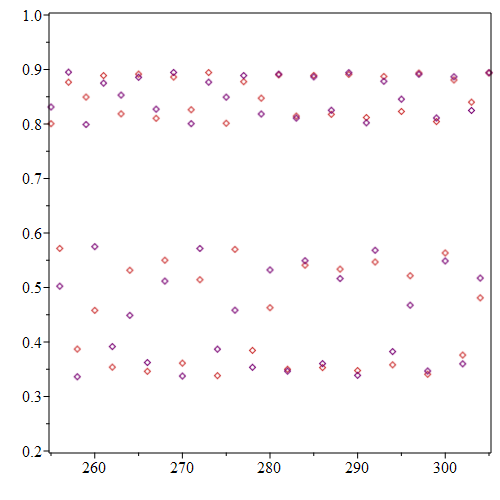
\includegraphics[scale=0.4]{butterfly2.png}
	\end{minipage}
	\hfill
	\begin{minipage}{0.2\textwidth}
		\textcolor{orange}{$ r=0.500 $}\\\textcolor{Plum}{$ r=0.505 $}
	\end{minipage}
	\caption{A plot for later $n$ that shows how small changes in the starting values of the period doubling sequence result in drastically different outcomes}
	\label{fig:mobFix}
\end{figure}
We can also see this behaviour continually for most $n$ after the chaotic threshold. It is important to remember that this is not random though -- the behaviour is still \textbf{deterministic} in that given the starting conditions, we can find the value of any term in the sequence.
\newpage
\section{Iterative Complex Sequences in the Form $z_{n+1} = {z_n}^2+c$}\label{s_zn}
In this section, I will be exploring sequences in the form $z_{n+1} = {z_n}^2+c$, focusing almost entirely on the concept of keep sets and escape sets.\\
First, we define the keep set, $K$, of this sequence as 
\begin{gather*}
K=\left\{z_0:\abs{z_n}<t_{\mathrm{max}}\quad\mathrm{as}\quad n\rightarrow\infty\right\} \\
\scalebox{0.8}{$\mathrm{where}\;0<t_{\mathrm{max}}<\infty$}
\end{gather*}
In context, $t_{\mathrm{max}}$ is a \textbf{threshold} value -- if the values of the sequence stay less than our set threshold value, then the starting value $z_0$ gets added to the set $K$. $t_{\mathrm{max}}$ is \textbf{independent} of $n$. \\
Similarly, the escape set, $E$ is defined as
\[E=\left\{z_0:\abs{z_n}>t_{\mathrm{max}}\quad\mathrm{as}\quad n\rightarrow\infty\right\}\]
Any values that satisfy this are then added to the set $E$
\subsubsection{Application to a Python 3.x.x program}
Whilst other programs have been left to the appendix without any explanation, I believe this program requires some context and explanation.
The Python implementation that I have written is as follows;
	\begin{lstlisting}[language=python]
yt_vals = []; yf_vals = []; xt_vals = []; xf_vals = []; xu_vals = []; yu_vals = []
import matplotlib.pyplot as plt
tolerance = 1; u_threshold = 100; l_threshold = 0.0000001
scan_resolution = 2000; complex_iters = 1000
c = complex(-1, 0)
absx = 2; absy = 1
for n in range(0, scan_resolution+1):
	x = xmin + n * 2 * absx / scan_resolution
	for m in range(0, scan_resolution+1):
		y = ymin + m * 2 * absy / scan_resolution
		z = complex(x, y)
		try:
			for i in range(complex_iters):
				z1 = pow(z, 2) + c
				z = z1
				if abs(z1) > u_threshold:
					break
				elif abs(z1) < l_threshold:
					break
				elif abs(z1) < tolerance:
					xu_vals.append(x)
					yu_vals.append(y)
				elif abs(z1) > tolerance:
					xf_vals.append(x)
					yf_vals.append(y)
				z1 = pow(z, 2) + c
				z = z1
				if abs(z1) < tolerance:
					xu_vals.append(x)
					yu_vals.append(y)
		except:
			xf_vals.append(x)
			yf_vals.append(y)
plt.plot()
plt.scatter(xf_vals, yf_vals, c = 'orchid', s = 0.1)
plt.scatter(xu_vals, yu_vals, c = 'green', s = 0.1)
plt.savefig('foo2.png', bbox_inches='tight',dpi=1700)
	\end{lstlisting}
In Python, it would not be possible to find the sets as $n\rightarrow\infty$, as Python is neither symbolic nor does it have the computational resources to do it numerically. Instead, we must specify our own value for the number of times that the sequence is iterated -- done in practice with the variable \texttt{complex\_iters}. With this, the code will take a given starting value and iterate it \texttt{complex\_iters} times before moving on to a new starting value. Starting values are calculated with the lines;
\begin{center}
	\texttt{x = xmin+n*2*absx/scan\_resolution}\quad and\quad \texttt{y=ymin+m*2*absy/scan\_resolution}
\end{center}
This has the effect of using \texttt{scan\_resolution} to specify the number of pixels between the positive and negative \texttt{absx} and \texttt{absy} -- it does this by taking the lowest values and adding fractions of the total length of the view area, splitting the $x, y$ plane equally into a grid of pixels for us to work with. The $x,\;y$ point then gets added to an array relating to its set condition (the set K or the set E). We then see the use of the \texttt{matplotlib} library from Python used to interpret these points as a scatter plot, with each set having its own colour -- `orchid' for an escaping point and 'green' for an an attracting point. This results in a pixel grid representing the $x,\;y$ plane in which we can see the set that each starting colour belongs to. \\
Without any optimization and \texttt{scan\_resolution = 2000; complex\_iters = 1000}, my \texttt{pythonw.exe} uses 8GiB of RAM and takes $\approx$ 30 minutes to complete -- optimization is needed for this code before attempting to compute more pixels or more iterations.
My optimisations come from the conditional statements;
\begin{center}
	\texttt{if abs(z1) > u\_threshold:}\quad and\quad \texttt{if abs(z1) < l\_threshold:}
\end{center}
Both of which result in a break from the surrounding iteration loop. This uses \texttt{u\_threshold} and \texttt{l\_threshold} to assume that if $z_n$ drops either above or below the threshold, then $z_n$ will continue to then tend towards either infinity or 0 respectively -- we then move on to a different $x_0$. This means that we no longer have to compute up to the value of \texttt{complex\_iters} for every starting point as many values will hit $0+0i$ or go above the threshold after many less iterations than the max that we allocated. Whilst it speeds up the execution quite a lot, this optimisation is at the expense of quality; with edges looking more smooth than they usually would as we are cutting a lot of detail away.\\
A few examples of figures can be seen on the next page
\newpage
\begin{figure}[H]
	\centering
	\begin{minipage}{0.725\textwidth}
		\centering
		\hfill
		\centering
		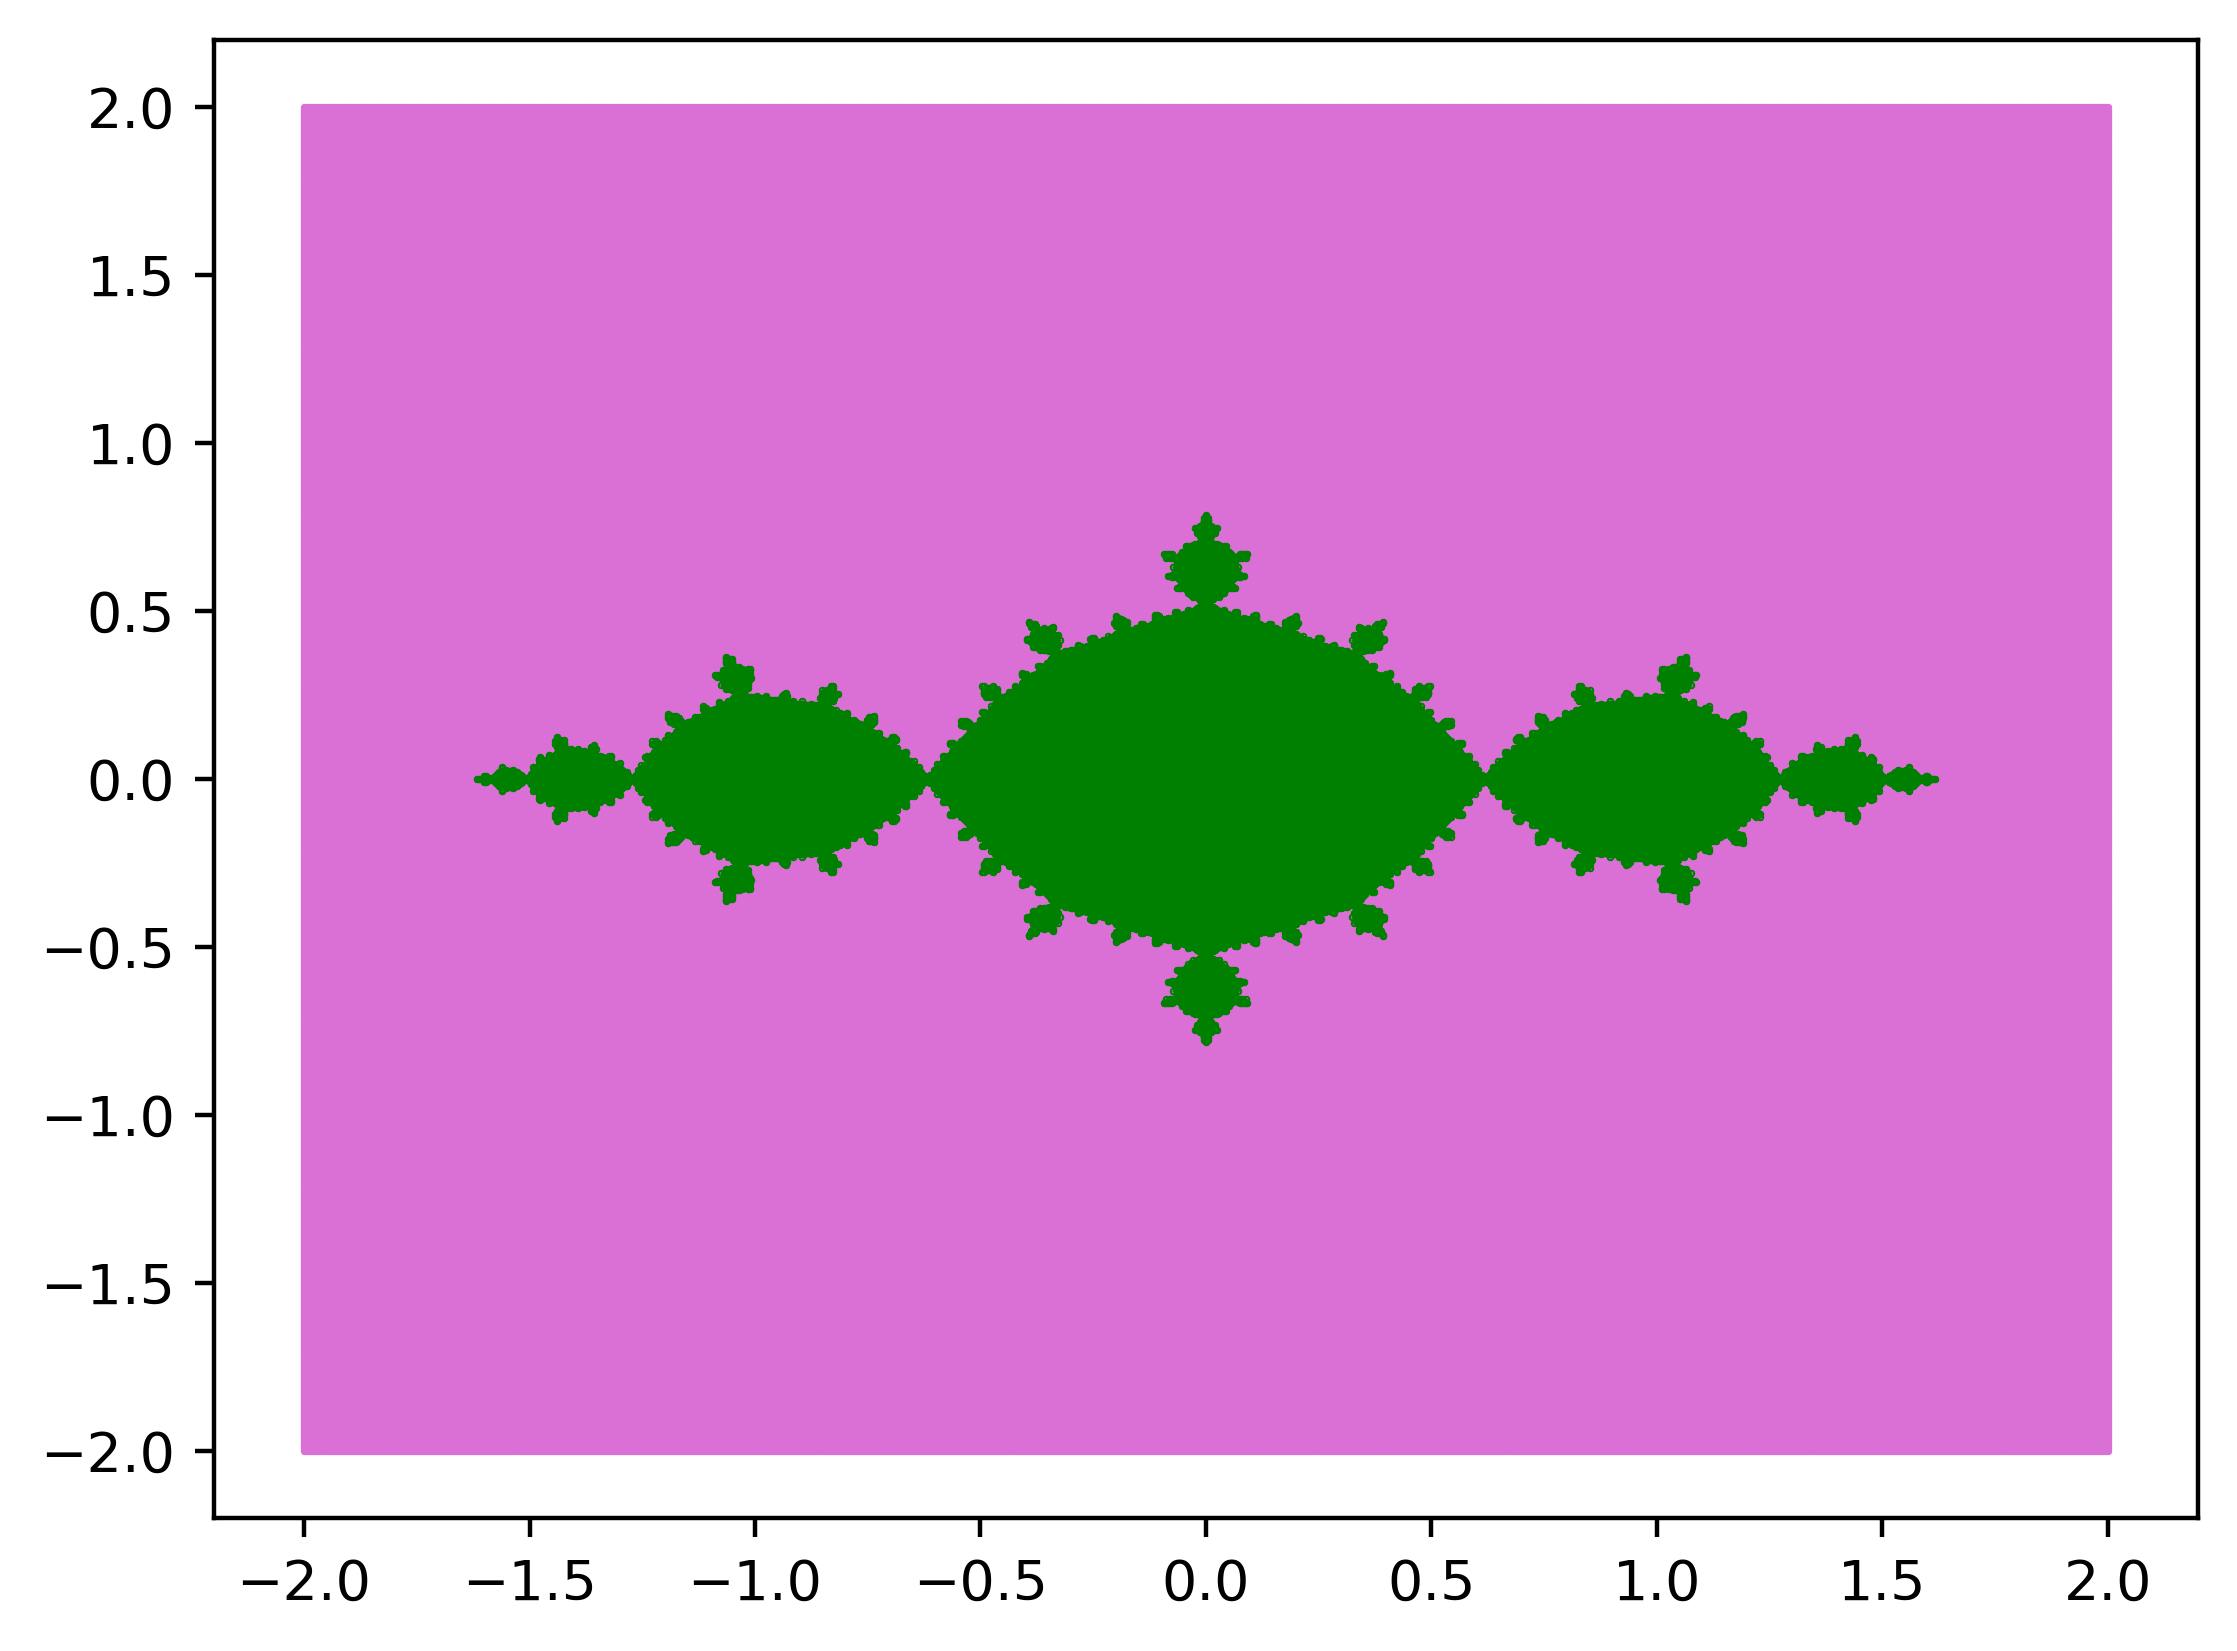
\includegraphics[scale=0.6]{m1i0.png}
	\end{minipage}
	\hfill
	\begin{minipage}{0.2\textwidth}
		$c=-1+0i$
	\end{minipage}
	\caption{Keep and escape sets shown in the $x,\;y$ plane, with the $y$-axis as the complex part}
	\label{fig:mobAsmp}
\end{figure}
\begin{figure}[H]
	\begin{minipage}{0.725\textwidth}
		\hfill
		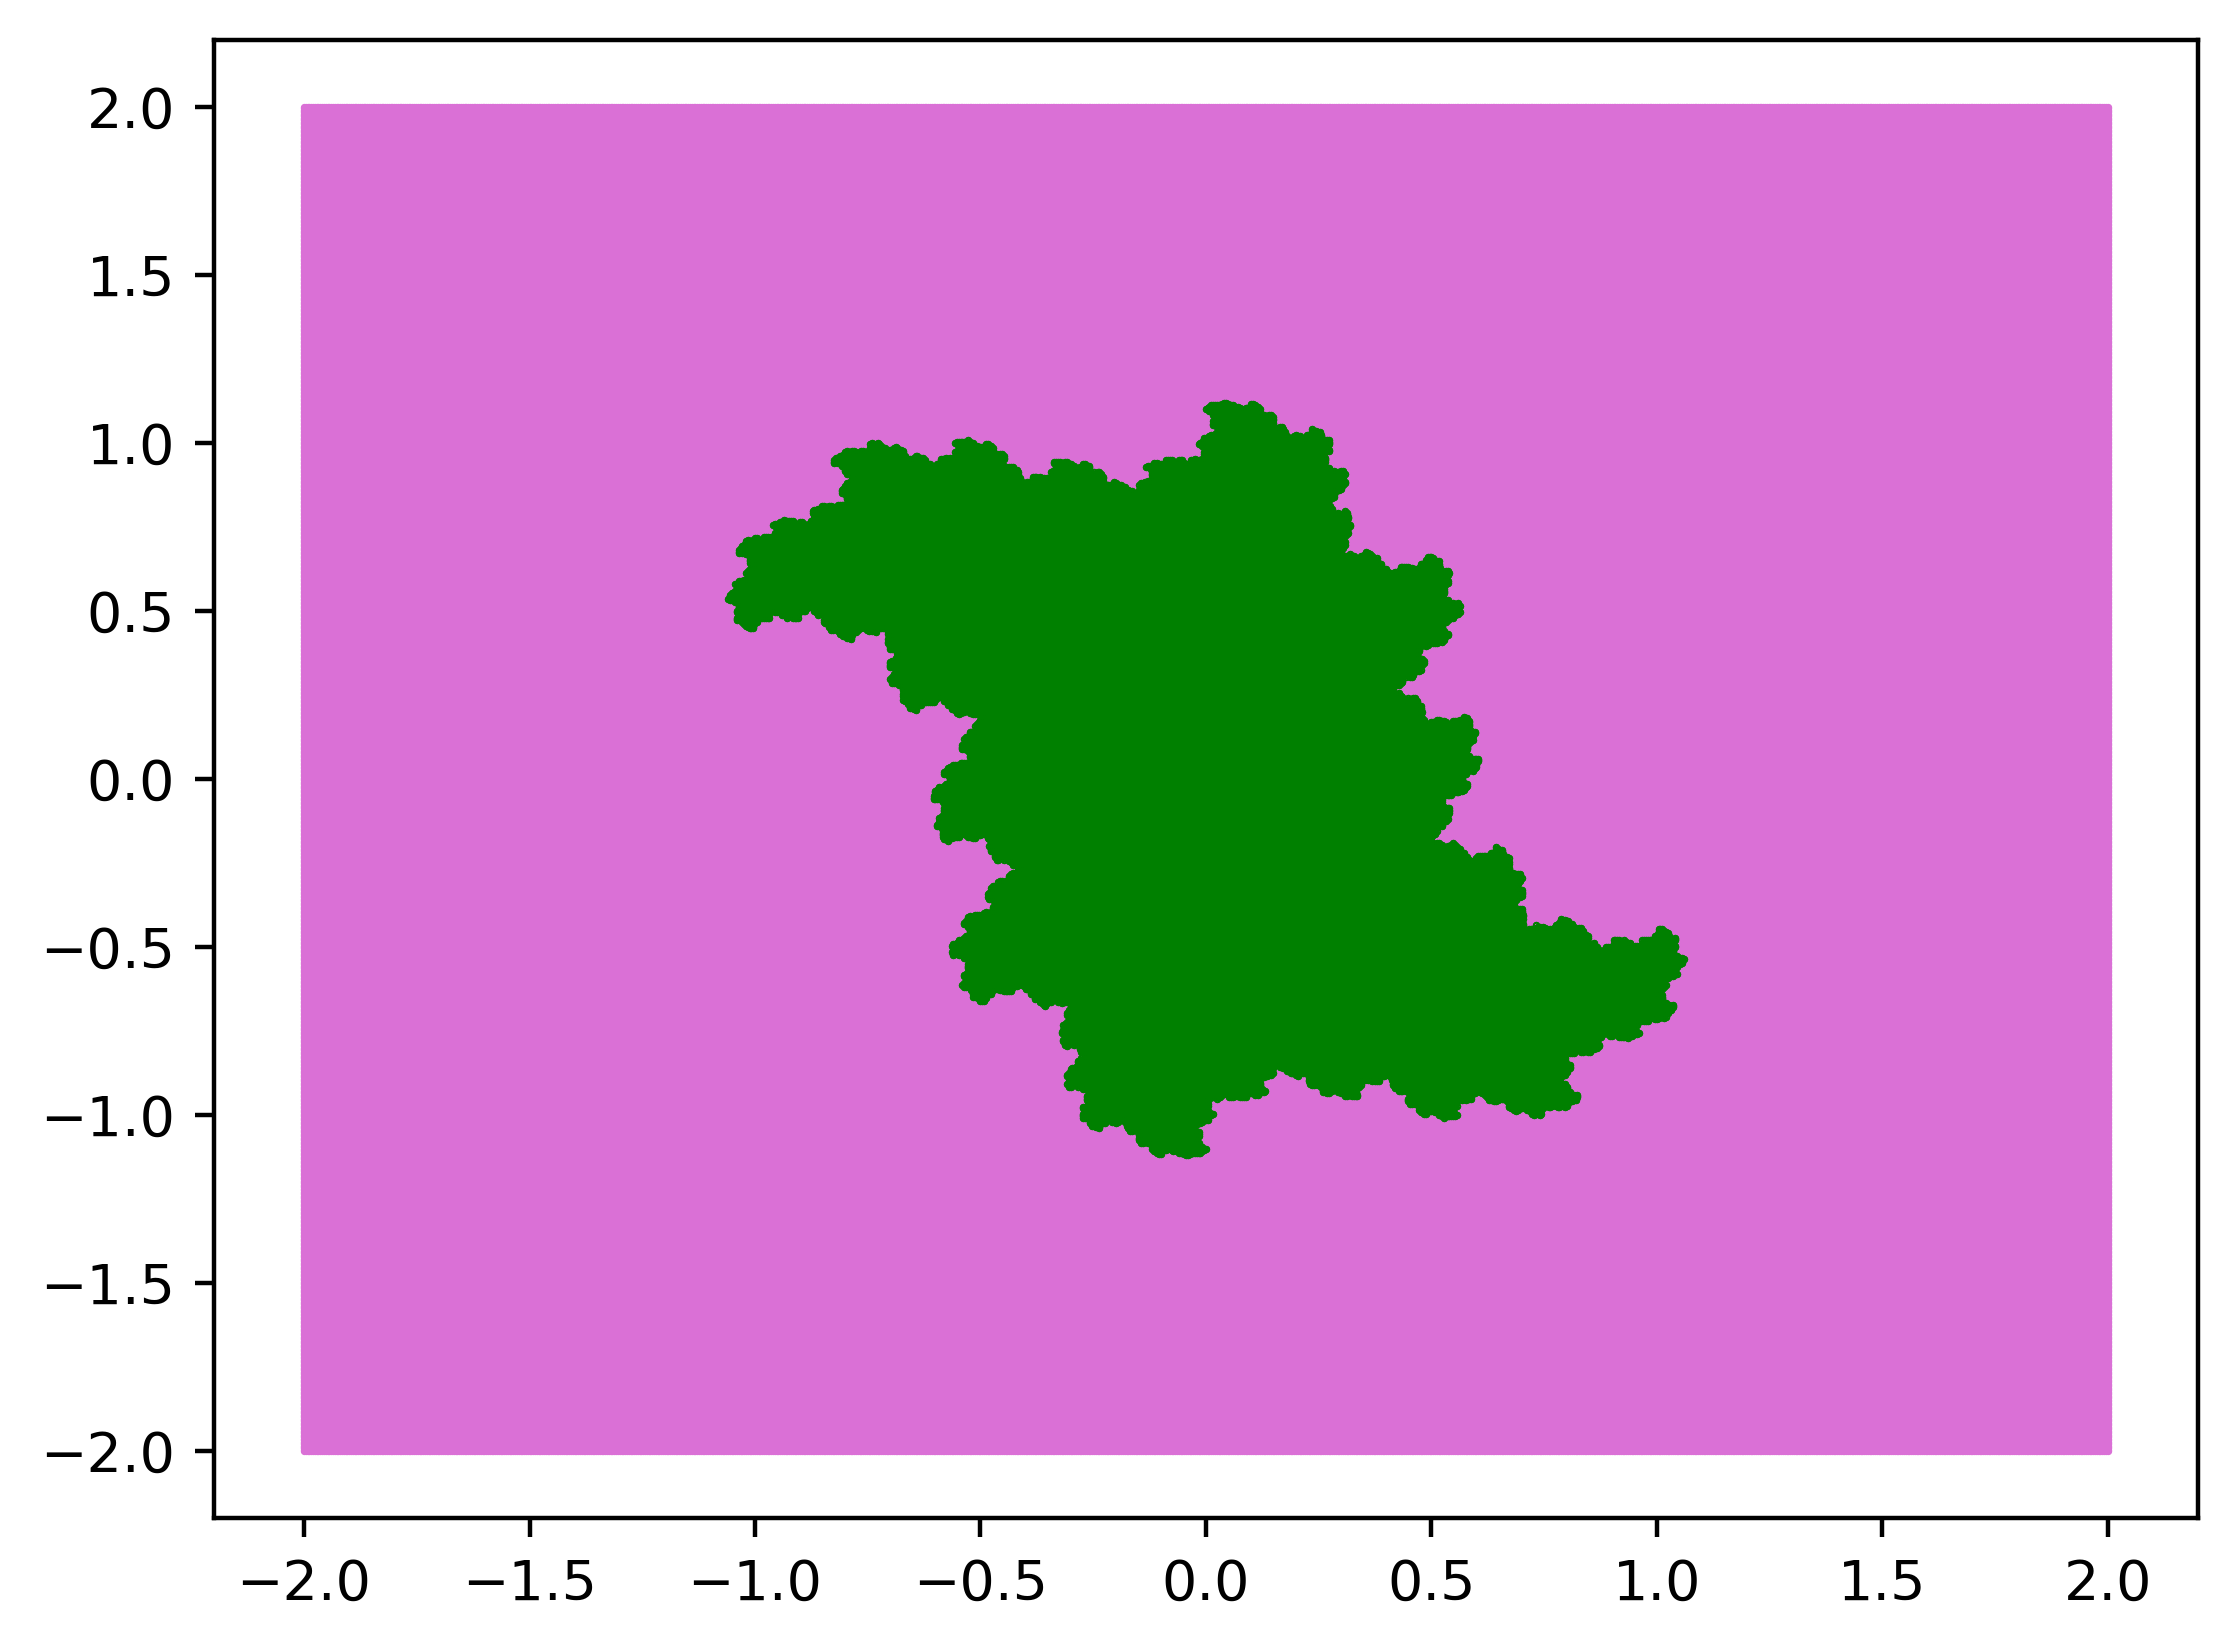
\includegraphics[scale=0.6]{02i045.png}
	\end{minipage}
	\hfill
	\begin{minipage}{0.2\textwidth}
		$c=0.2+0.45i$
	\end{minipage}
	\caption{Keep and escape sets shown in the $x,\;y$ plane, with the $y$-axis as the complex part}
	\label{fig:mobAsmp}
\end{figure}
\begin{figure}[H]
	\begin{minipage}{0.725\textwidth}
		\hfill
		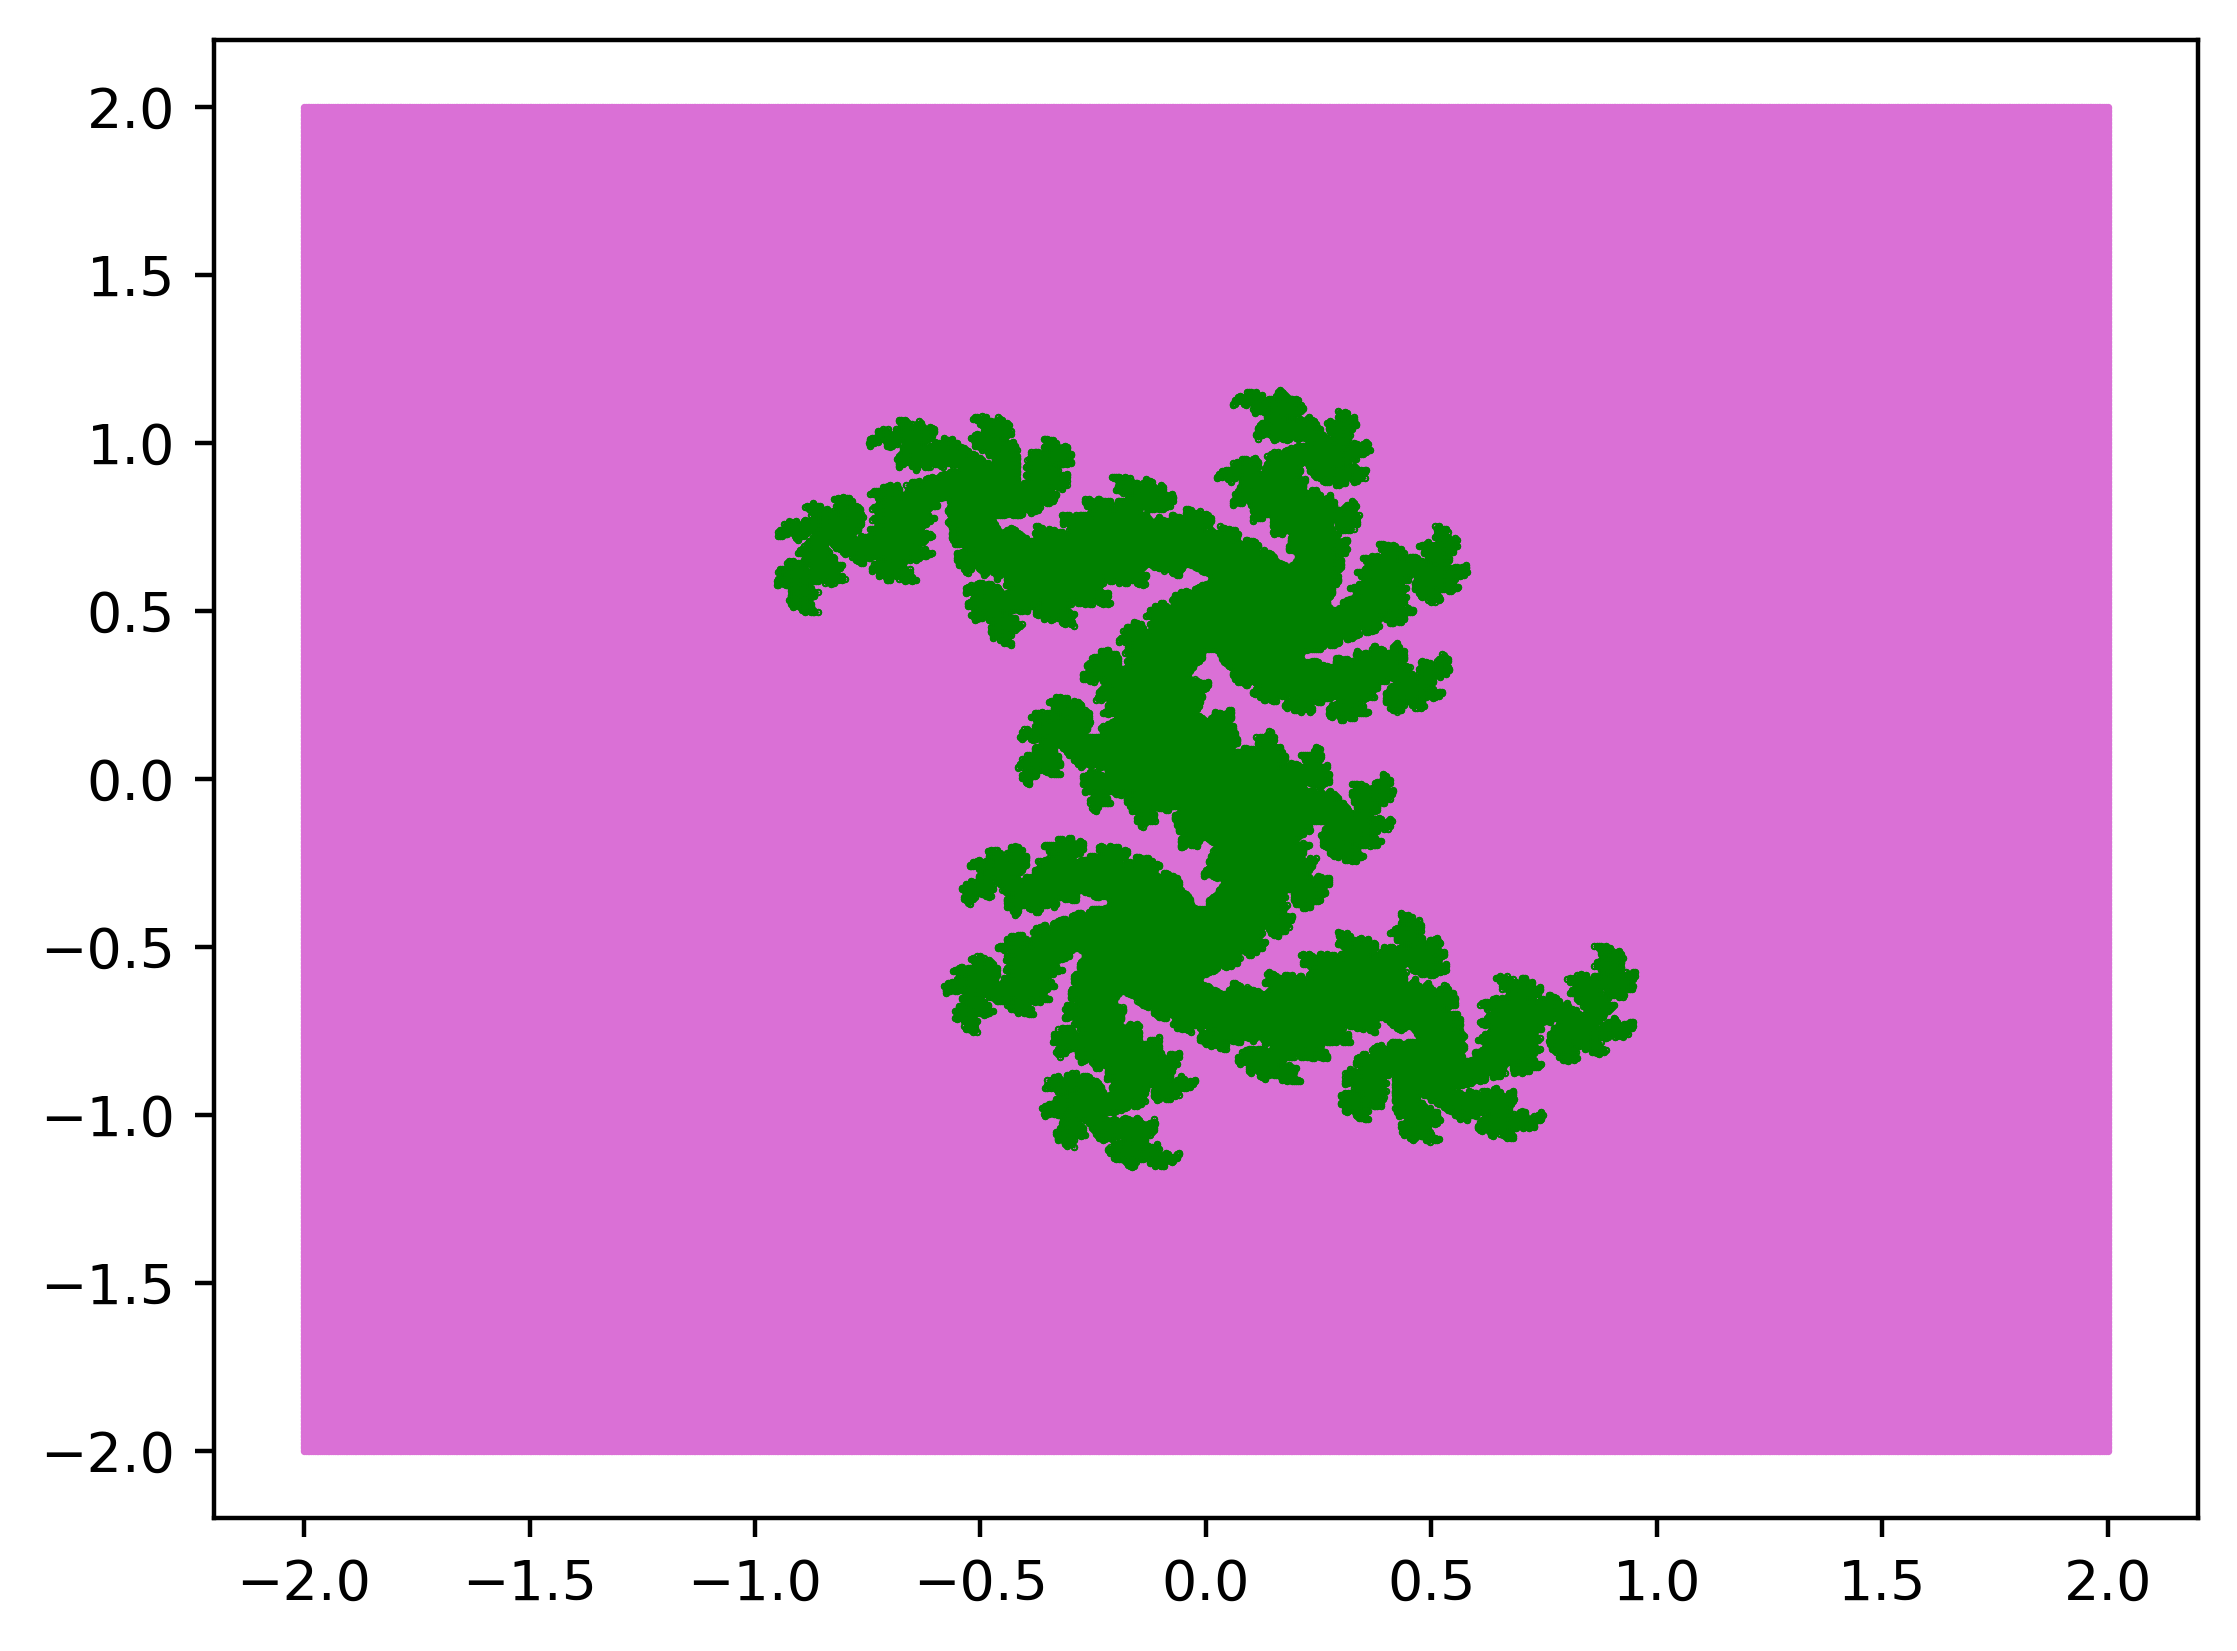
\includegraphics[scale=0.6]{037i036.png}
	\end{minipage}
	\hfill
	\begin{minipage}{0.2\textwidth}
		$c=0.37+0.36i$
	\end{minipage}
	\caption{Keep and escape sets shown in the $x,\;y$ plane, with the $y$-axis as the complex part}
	\label{fig:mobAsmp}
\end{figure}
%%%%%%%%%%%%%%%
\subsection{The case for $c = -2$}
When we graph the sets for $c=-2$, we get the result shown below
\begin{figure}[H]
	\centering
	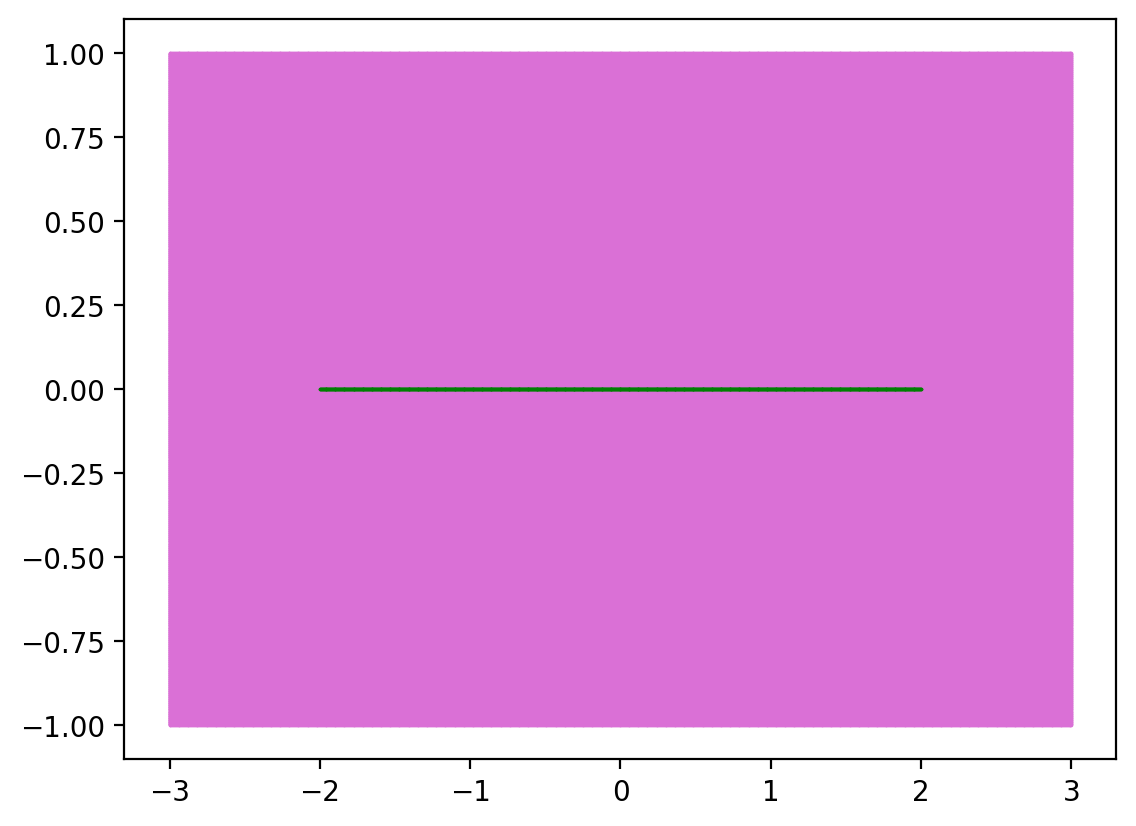
\includegraphics[scale=0.6]{-2i0.png}
	\caption{The keep and escape sets for $c=-2$}
\end{figure}
The keep set is a line segment such that 
\[-2\leq\Re(K)\leq2,\quad\Im(K)=0\]
%\[K=\left\{x_0:\abs{x_n}\le2\quad\mathrm{as}\quad n\rightarrow\infty,\quad K\in\mathbb{R}\right\}\]
Plainly, this is a line segment that exists only on the real plane. This result differs from the filled shapes that we saw in previous examples.
\newpage
\subsubsection{A proof for the result for $c = -2$}
There are 3 parts to this proof;
Firstly, if $z_0$ lies in the line segment $K$, then $z_n$ will also lie within $K$, this can be shown by the following;
\begin{equation*}
	\begin{array}{ccccc}
	-2 & \le & z_0 & \le & 2 \\[2pt]
	-2  & \le &  {z_0}^2-2  & \le & 2 \\[2pt]
	-2 & \le &   z_1   & \le & 2
	\end{array}
\end{equation*}
It follows from repeated iterations that $z_n$ will stay in the interval $[-2,2]$. \\
We must then show that if $z_0$ does not lie in $K$, $z_n$ must also not lie within $K$. We can do this by showing that if $z_{n+1}$ lies in $K$, $z_n$ must also be in $K$ (the contrapositive is also true; $z_0$ is not in $K$, so $z_n$ will not be in $K$)
\begin{align*}
	\shortintertext{Given that $z_n = x+iy$}
	z_{n+1} & = (x+iy)^2-2     \\
	        & = x^2+2ixy-y^2-2
\end{align*}
For this to lie in $K$, it is implied that either $x=0$ or $y=0$ to satisfy that $K$ is the interval $[-2,2]$. This is due to the fact that we know that $K$ never has any imaginary parts.
Consider $x=0$;
\[-2\le -y^2-2 \le 2\]
This implies that $y=0$. Now consider the case that $y=0$ initially.
\begin{equation*}
	\begin{array}{ccccc}
		-2 & \le & x^2-2 & \le & 2 \\[2pt]
		0  & \le &  x^2  & \le & 4 \\[2 pt]
		-2 & \le &   x   & \le & 2
	\end{array}
\end{equation*}
This shows us that for $z_{n+1}$ to lie in $K$, $z_n$ must lie in $K$ -- eventually showing that $z_0$ was in $K$. We can then deduce that if $z_0$ is not in $K$, it will never be apart of $K$ in future iterations.\\
We must then show that not only does $z_n$ never return to $K$, but that it tends to infinity also.
Firstly, let $z$=$w+\frac{1}{w}$

	\begin{align*}
		z & =w+\frac{1}{w} \\
		wz                 & =w^2+1         \\
		0                  & =w^2-wz+1      \\ \shortintertext{It folows that there are two solutions, but we know that $w w^{\prime}=1$ due to how $z$ is defined in terms of $w$ above -- and also that $\abs{w}\abs{w^{\prime}}=1$}
	\end{align*}
Consider that $\abs{w}=1$
	\begin{align*}
		\abs{w}     & = 1                          \\
		w           & = \cos{\theta}+i\sin{\theta} \\
		\frac{1}{w} & = \cos{\theta}-\sin{\theta}  \\
		z           & =2\cos{\theta}
	\end{align*}
It can be deduced from this that as $\cos{\theta}$ has a range of $-1$ to $1$, $z\in[2,2]$.\\
Consider\footnote{Choosing $\abs{w}<1$ gives us a similar result -- only tending towards zero instead of infinity} instead that $\abs{w}>1$, there will always be a $w$ which satisfies as $ww^\prime=1$.
\begin{align*}
	{z_n}^2-2 & = z_{n+1}                                    \\
	          & = w_{n+1}+\frac{1}{w_{n+1}}                  \\
	          &                                              \\
	{z_n}^2-2 & = \left[w_{n+1}+\frac{1}{w_{n+1}}\right]^2-2 \\
	          & = {w_{n}}^2+\frac{1}{{w_{n}}^2}
\end{align*}
Equating the results for ${z_n}^2-2$ we can deduce that
\begin{align*}	          
	0 & = w_{n+1}+\frac{1}{w_{n+1}}-{w_{n}}^2-\frac{1}{{w_{n}}^2}          \\[2pt]	
	0 & = {w_{n+1}}^2+1-{w_{n}}^2 w_{n+1}-\frac{w_{n+1}}{{w_{n}}^2}        \\[3pt]
	0 & = {w_{n+1}}^2{w_{n}}^2+{w_{n}}^4-{w_{n}}^2w_{n+1}-w_{n+1}		   \\[6pt]
	0 & = \left({w_n}^2w_{n+1}-1\right)\left(w_{n+1}-{w_n}^2\right)  	
\end{align*}
Which gives us the solutions for $w_{n+1}$ as
\[w_{n+1}=\left\{{w_n}^2,\quad\frac{1}{{w_n}^2}\right\}\]
This shows us that the sequence squares each iteration. As $\abs{w_n}>1$, $w_n$ will approach infinity as $n$ increases. The second solution can be ignored.
If $w_n$ approaches infinity, then $z_n$ will approach infinity also -- due to the fact that 
\[\lim_{w_n \to \infty} \left[w_n+\frac{1}{w_n}\right] = \infty\]
As $z_n$ was previously defined as $\left[w_n+\frac{1}{w_n}\right]$, it is obvious that $z_n$ also tends to infinity and will never go back towards the keep set -- $z_0$ therefore belongs to the escape set.
\newpage
\subsection{Cycles represented on the keep/escape diagram}
Unsurprisingly, cycles occur in this complex sequence also. A 3-cycle, for example, has the property that
\[f^3(z)-z=0\]
Solving this similarly to before with a given value for $c$ will give us all of the fixed points for the function and also the solutions to each value in the 3-cycle. Interestingly, if we take both of the 3-cycles\footnote{There are 2 possible cycles that occur in complex conjugate pairs.} then the resulting plot will show them on the boundary of the keep set. The example below gives the 3-cycles for $c=-1$ where the blue points are the conjugates of the red points. 
\begin{figure}[H]
	\centering
	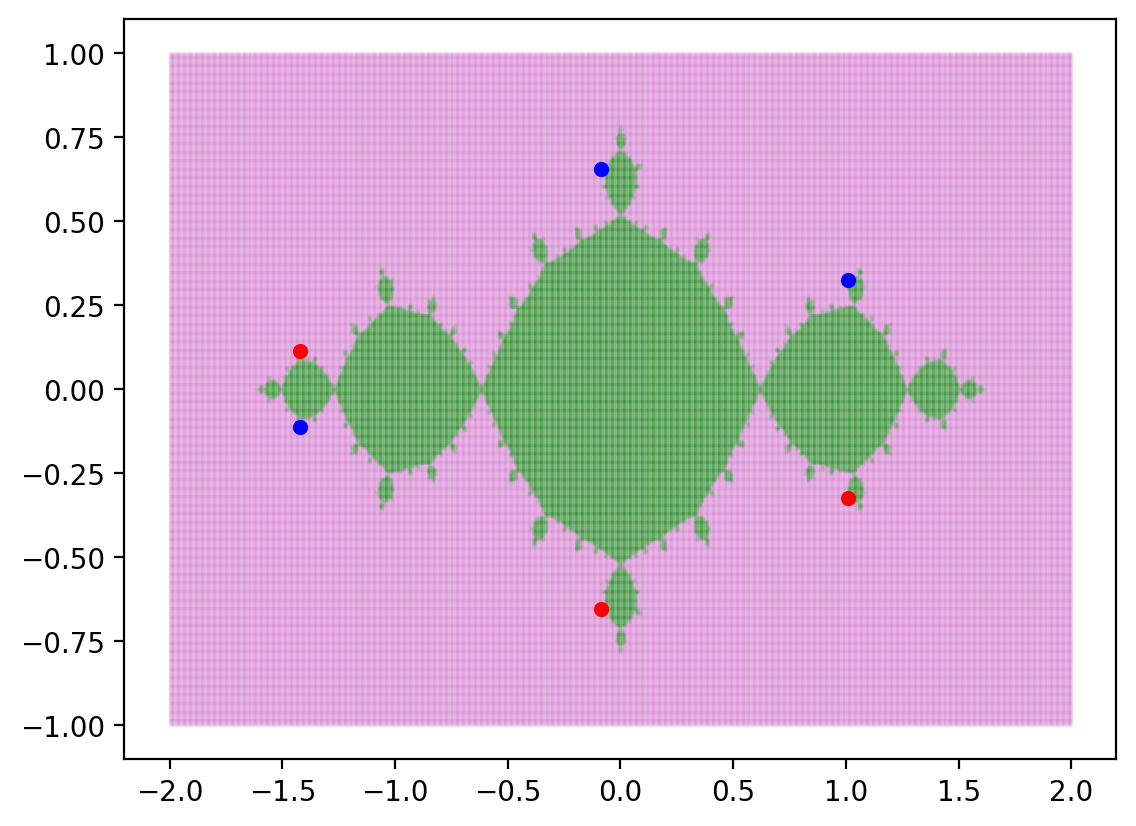
\includegraphics[scale=0.8]{zCycles.png}
	\caption{The keep and escape sets for $c=-2$}
\end{figure}
This behaviour can be seen on all cycle lengths, with the boundary of the sets being where all the cycles lie, as the values tend toward neither 0 nor infinity. It would be ideal to color this boundary with a different colour -- however due to the limited number of points that my implementation scans, it is highly unlikely that the starting points will be the exact starting point needed for an $n$-cycle.\\
%A better solution to visualise these sets with more detail would be to colour not based on the set that the starting point lies in -- but to colour based on the number of iterations needed for that starting point to go above a certain threshold (or below a threshold for $x_0$ values that do not tend toward infinity.\\
%With this new colouring scheme, we can see more detail about the rates at which $x_0$ tend towards either zero or infinity (and also the cyclic values of $x_0$);

\newpage
\section{Acknowledgements}
I would like to thank the Nuffield Foundation for making this project possible by offering me a place on the programme this summer; it has helped me to learn about research skills and how a good research paper is presented. This project has also helped me to develop my communication skills -- working out how to present the information in a manner understandable by as many readers as possible. The communication skills that I have developed also extend to how I speak with the regional co-ordinators and my project supervisor.\\
I would like to thank my project supervisor, Peter Giblin from the University of Liverpool. They have helped me from start to finish; aiding me in understanding the key concepts of the topics researched and providing feedback on any drafts of the report that I have sent. Not to mention that all of this was in different circumstances this year to to COVID-19 -- all communication was done over video calls instead of in person, making the whole process more difficult at every stage. Despite this, I have enjoyed myself at all stages of the programme.
\newpage
\bibliography{biblio}
\newpage
\section{Appendix}
\subsection{Programs}
\subsubsection{Maple program to generate the roots of unity graphic}
\begin{lstlisting}
with(plots);
with(plottools);
with(Statistics);
circleplot:=implicitplot(x^2+y^2=1,x=-1.5..1.5,y=-1.5..1.5);
t1:=textplot([1/2,sqrt(3)/2,'typeset'([lambda[1]/lambda[2]])],align={'above','right'});
t2:=textplot([-1/2,-sqrt(3)/2,'typeset'([lambda[1]/lambda[2]]^2)],align={'below','left'});
t3:=textplot([1,0,'typeset'([lambda[1]/lambda[2]]^3)],align={'below','right'});
display(t1,t2,t3,line([0,0],[1/2,sqrt(3)/2],thickness=3),line([0,0],[-1/2,-sqrt(3)/2],thickness=3),line([0,0],[1,0],thickness=3),circleplot,view=[-1.5..1.5,-1.5..1.5],axes=normal,scaling=constrained);
\end{lstlisting}
\subsubsection{A Maple Program to generate cobweb plots used in the Mobius sequence section}
\begin{lstlisting}
restart:
a:=a:b:=b:c:=d:d:=d:start:=start:endd:=endd:iters:=iters:
with(plots):with(plottools):
f:=x->(a*x+b)/(c*x+d);
f:=proc(x)->(a*x+b)/(c*x+d)endproc
plot1half:=plot([x,f(x),x=start..endd],color=red):
plot2half:=plot([x,f(x),x=start..endd],color=red):
plot3x:=plot([x,x,x=start..endd]):
i:=1:y0:=0:y1:=0.1:x0:=3:
while i<iters do
	y0:=evalf(f(x0)):
	line1[i]:=line([x0,x0],[x0,y0]):
	line2[i]:=line([x0,y0],[y0,y0]):
	x0:=y0:y1:=evalf(f(y0)):
	i:=i+1:
end do:
display({plot1half,plot2half,plot3x,seq(line1[i],i=1..iters),seq(line2[i],i=1..iters)});
\end{lstlisting}
\subsubsection{A Maple program to generate cobweb plots for the period doubling sequence}
\begin{lstlisting}
restart:
a:=starting_a
with(plots):with(plottools):
x0:=0.5:
f:=x->a*x*(1-x):
i:=1:y0:=0:y1:=0.1:
while i<1500 do
	y0:=evalf(f(x0)):
	line1[i]:=line([x0,x0],[x0,y0]):
	line2[i]:=line([x0,y0],[y0,y0]):
	x0:=y0:y1:=evalf(f(y0)):
	i:=i+1
end do:
plot1:=plot([x,f(x),x=0..1],color=red):
plot3:=plot([x,x,x=0..1]):
display({plot1,plot3,seq(line1[i],i=1..1499),seq(line2[i],i=1..1499)});
\end{lstlisting}
\subsubsection{A Maple program to generate 7-cycle $a,\;b,\;d$ surfaces}
\begin{lstlisting}
restart;
with(plots);
f:=x->a*x*(1-x);
solve(f(f(x))-x=0,x);
cycdiff:=diff(f(f(x)),x);
cycdiff:=a^2*(1-x)*(1-a*x*(1-x))-a^2*x*(1-a*x*(1-x))+a^2*x*(1-x)*(-a*(1-x)+a*x)
fsolv:=solve(f(f(x))-x=0,x);
f2:=x->a^2*(1-x)*(1-a*x*(1 -x))-a^2*x*(1-a*x*(1-x))+a^2*x*(1-x)*(-a*(1-x)+a*x);
ab:=plot(subs(x=fsolv[4],f2(x)),a=0..40);
ac:=implicitplot((x-3)*(x+(-1-sqrt(6)))=0,x=0..4,y=-4..4);
solve(subs(x=fsolv[3],f2(x))=-1,a);
display(ab, ac, view = [2 .. 4, -4 .. 4]);
\end{lstlisting}
\subsubsection{A Maple program to find the limit of a 2-cycle in the period doubling sequence}
\begin{lstlisting}
restart;
with(plots);
f := x -> a*x*(1 - x);
solve(f(f(x)) - x = 0, x);
simplify(f(f(x)) - x);
cycdiff := diff(f(f(x)), x);
fsolv := solve(f(f(x)) - x = 0, x);
f2 := x -> a^2*(1 - x)*(1 - a*x*(1 - x)) - a^2*x*(1 - a*x*(1 - x)) + a^2*x*(1 - x)*(-a*(1 - x) + a*x);
ab := plot(subs(x = fsolv[4], f2(x)), a = 0 .. 40);
ac := implicitplot((x - 3)*(x + (-1 - sqrt(6))) = 0, x = 0 .. 4, y = -4 .. 4);
solve(subs(x = fsolv[3], f2(x)) = -1, a);
\end{lstlisting}
\newpage
\subsubsection{A Maple program to generate Julia sets for the iteration of $z_{n+1}={z_n}^2+c$}
\begin{lstlisting}
import matplotlib.pyplot as plt
import math as m
yt_vals = []
yf_vals = []
xt_vals = []
xf_vals = []
xu_vals = []
yu_vals = []
tolerance = 1
threshold = 25
scan_resolution = 1000
complex_iters = 400
c = complex(-1, 0)
absx=2
absy=1
xmin = -absx
xmax = absx
ymin = -absy
ymax = absy
for n in range(0, scan_resolution+1):
	x = xmin + n * (xmax - xmin) / scan_resolution
	for m in range(0, scan_resolution+1):
		y = ymin + m * (ymax - ymin) / scan_resolution
		z = complex(x, y)
		try:
			for i in range(complex_iters):
				z1 = pow(z, 2) + c
				z = z1
				if abs(z1)>threshold:
					#print('x: {}\ny: {}\ni:{}\nz: {}'.format(str(x),str(y),str(i),str(abs(z1))))
				break
				if abs(abs(z1) - tolerance)<0.4:
					xt_vals.append(x)
					yt_vals.append(x)
				elif abs(z1) < tolerance:
					xu_vals.append(x)
					yu_vals.append(y)
				elif abs(z1) > tolerance:
					xf_vals.append(x)
					yf_vals.append(y)
				elif z == (nan+nanj):
					xf_vals.append(x)
					yf_vals.append(y)
				z1 = pow(z, 2) + c
				z = z1
				if abs(z1) < tolerance:
					xu_vals.append(x)
					yu_vals.append(y)
			except:
				xf_vals.append(x)
				yf_vals.append(y)
plt.plot()
plt.scatter(xf_vals, yf_vals, c = 'orchid', s = 0.1)
plt.scatter(xu_vals, yu_vals, c = 'green', s = 0.1)
plt.savefig('foo.png', bbox_inches='tight')
#plt.scatter(xt_vals, yt_vals, c = 'green', s = 5)
#plt.scatter(x2_vals, y2_vals, c = 'black', s = 10)
#plt.scatter(x3_vals, y3_vals, c = 'black', s = 10)


\end{lstlisting}
\newpage	
\subsubsection{A Python program to plot the differences between the value of the fixed point and the term of the sequence, in respect to the $n$\textsuperscript{th} iteration}
\begin{lstlisting}
restart;
with(ArrayTools);
with(Statistics);
with(plots);
with(plots);
with(plottools);
x0:=0.5;
xres:=50;
a:=2.79:x0:=0.5:i:=1:y0:=0:y1:=0.1:
f:=x->a*x*(1-x):
fixd:=fsolve(f(x)=x);
i:=1:y0:=0:y1:=0.1:
xdata:=Array([]);
ydata:=Array([]);
while i<xres do
	y0:=evalf(f(x0)):
	p:=fixd[2]-y0:
	Append(xdata,i):
	Append(ydata,p):
	x0:=y0:y1:=evalf(f(y0)):
	i:=i+1
end do:
conv21:=ScatterPlot(xdata,ydata,lowess=false,degree=2,color='orange');
a:=2.89:x0:=0.5:i:=1:y0:=0:y1:=0.1:
f:=x->a*x*(1-x):
fixd:=fsolve(f(x)=x);
xdata:=Array([]);
ydata:=Array([]);
while i<xres do
	y0:=evalf(f(x0)):
	p:=fixd[2]-y0:
	Append(xdata,i):
	Append(ydata,p):
	x0:=y0:y1:=evalf(f(y0)):
	i:=i+1
end do:
conv26:=ScatterPlot(xdata,ydata,lowess=false,degree=2,color='purple');
a:=2.99:x0:=0.5:i:=1:y0:=0:y1:=0.1:
f:=x->a*x*(1-x):
fixd:=fsolve(f(x)=x);
xdata:=Array([]);
ydata:=Array([]);
while i<xres do
	y0:=evalf(f(x0)):
	p:=fixd[2]-y0:
	Append(xdata,i):
	Append(ydata,p):
	x0:=y0:y1:=evalf(f(y0)):
	i:=i+1
end do:
conv29:=ScatterPlot(xdata,ydata,lowess=false,degree=2);
display(conv21,conv26,conv29,labels=[n,x[n]],line([0,0],[50,0]));
\end{lstlisting}
%\listoffigures
\end{document}